\chapter{复数}
\section{引言——数系的发展与复数的起源}
数的概念及运算是从生产和科学研究的实践中产生和发展起来的。截至目前,同学们学过的数系是下表中实线画出的部分:
\begin{center}
    \begin{tikzpicture}[>=stealth]
\node (A) at (0,.5)[text width=1.5cm, align=center]{复数集\\($\mathbb{C}$)}; 
\node (B1) at (1.6,1.5)[text width=1.5cm, align=center]{实数集\\($\mathbb{R}$)}; 
\node (B2) at (1.6,-.5)[text width=1.5cm, align=center]{虚数集}; 
\node (C1) at (2.3,2.5)[right, text width=1.5cm, align=center]{有理数集\\($\Q$)}; 
\node (C2) at (2.3,1)[right, text width=5cm, align=center]{无理数集——无限不循环小数}; 
\node (D1) at (5,3)[text width=1.5cm, align=center]{整数集\\($\Z$)}; 
\node (D2) at (5,2)[text width=1.5cm, align=center]{分数集}; 
\node (E1) at (6.75,4)[text width=1.5cm, align=center]{自然数集\\($\N$)}; 
\node (E2) at (6.75,3.25)[text width=1.5cm, align=center]{零}; 
\node (E3) at (6.75,2.5)[text width=1.5cm, align=center]{负数}; 
\node (F1) at (9,3)[text width=2.5cm, align=center]{循环小数\\(包括整数和有限小数)}; 
\draw[decorate, decoration={brace, amplitude=8pt}, dashed](1,-.5)--(1,1.75);
\draw[decorate, decoration={brace, amplitude=5pt}](2.5,1)--(2.5,2.75);
\draw[decorate, decoration={brace, amplitude=5pt}](4.35,2)--(4.35,3.25);
\draw[decorate, decoration={brace, amplitude=5pt}](6,2.25)--(6,4.5);
\draw[decorate, decoration={brace, amplitude=5pt}](7.75,4.5)--(7.75,1.75);
    \end{tikzpicture}
    \end{center}

正如表中所列出的,从正整数(自然数)集$\N$到实数集$\R$,数系已经经历了三次扩充(下表中实箭头表示的部分)。本章将研究第四次扩充(虚箭头表示的部分):
\begin{center}
\begin{tikzpicture}[>=stealth]
\node(A) at (0,0)[text width=2cm, align=center]{正整数集\\($\N$)} ;
\node(B) at (6,0)[text width=1.5cm, align=center]{整数集\\($\Z$)} ;
\node(C) at (10,0)[text width=1.5cm, align=center]{有理数集\\($\Q$)} ;

\node(D) at (4,-1.5)[text width=1.5cm, align=center]{实数集\\($\R$)} ;
\node(E) at (8,-1.5)[text width=1.5cm, align=center]{复数集\\($\mathbb{C}$)} ;

\draw[->](A)--node[text width=4cm, align=center]{第I次\\引进零和负数}(B);
\draw[->](B)--node[text width=2cm, align=center]{第II次\\引进分数}(C);
\draw[->](D)--node[text width=2cm, align=center]{第IV次\\引进虚数}(E);
\draw[->](0,-1.5)--node[text width=2cm, align=center]{第III次\\引进无理数}(D);
\end{tikzpicture}
\end{center}


“温故知新”,让我们先回顾一下前三次扩充的事实和规律.

\subsection{从数集上的元素看}
数集的每次扩充都是在原有数集的基础上引入新数,构造出一个新数集,且使原有的数集成为新数集上的一个真子集。也就是说,数集以\textbf{逐次包含}的方式扩充。

\subsection{从数集上的运算看}
在新数集上我们这样定义新的运算法则:一方面要使新法则运用到原有数集上时必须与原有数集上的运算结果相一致;另一方面我们还希望新法则能使原数集上的运算规律保持不变。例如,在有理数集上计算$(+5)+(+6)$的结果应与在算术(正有理数集)中计算$5+6$的结果相一致,而且我们还希望在算术中对加法和乘法成立的交换律、结合律和分配律能在有理数集上保持不变。也就是说,在原来数集上成立的算律,在扩充后的数集上希望它能继续成立。这是很重要的\textbf{数集扩充的原则}。

\subsection{从数集扩充的动力看}
数集的每次扩充既是度量的需要(这一点大家比较清楚),又是数学理论发展的需要(特别是解方程的需要)。例如:

方程$x+4=0$在自然数集上无解,而在扩充后的整数集上有唯一解$x=-4$;

方程$5x=3$,在整数集上无解,而在扩充后的有理数集
上有唯一解$x=\frac{3}{5}$(若不扩充数集,连这种最简单的一元一
次方程的理论也不能完整)。

方程$x^2=2$在有理数集上无解,在扩充后的实数集上有两个解$x=\pm\sqrt{2}$.

最早呼唤扩充实数集的问题是解二次方程。事实上,在实数集上不能提供二次方程的完整理论。如方程
\begin{equation}
    x^2=-1 \tag{1}
\end{equation}
在实数集上就没有解,因为任意实数的平方都不可能为负数。

摆在人们面前有两种选择:要么宣布方程(1)无解;要么沿着数集扩充的方向朝前走——引入新数,扩充实数集,使方程(1)有解。一些严峻的事实迫使人们选择了后者。于是在16世纪中叶,人们开始引入一个由等式
\begin{equation}
    i^2=-1  \tag{2}
\end{equation}
所定义的新数$i$(它显然不是实数)\footnote{$i$是英文单词imaginaries(虚的)的字头,瑞士大数学家欧拉首先用它表示虚数单位.
},它被称做虚数单位。这样,方程(*)至少有了一个根$i$。进而,根据数集扩充的原则,我们还规定实数可以和它进行四则运算,并且进行四则运算时,原有的加、乘算律仍然成立。于是自然造出了诸如$2i$, $3i$, $2+5i$这样一些新数。

应该指出:引进的新数$i$以及上面造出的形如$a+bi$($a,b\in\R$)的数,起初人们对它感到迷惑不解,特别是当$b\ne 0$时,认为这些都是“虚假的数”[这是因为当时人们习惯于把数作为某种计数手段,然而形如$a+bi\; (a,b\in\R,\; \text{且}b\ne 0)$的新数却起不到计数手段的作用],“虚数”正是由此而得名。

虚数诞生后,除了用来表示方程的解以外,一时尚找不
到更多的应用,因此发展十分缓慢。到了18世纪末叶,维塞尔(Wessel)、阿尔纲(Argand)和高斯(Gauss)几乎同时给这些新数以几何解释(见6.2节)以后,才在数学、物理的应用和研究中逐渐有了越来越多且越来越重要的用途,这进一步推动了人们研究的兴趣。19世纪初,高斯把形如$a+bi\; (a,b\in\R)$的数称为复数。如果说微积分的研究统治了18世纪的话,那么,19世纪数学家们的兴奋中心便是关于复数理论及其应用的研究。现在复数已经发展成为一门十分重要的基础数学分支——复变函数论,它是数学、物理和技术科学中有力的数学工具之一。

本章将学习复数的初步知识。

\section{复数的概念}
\subsection{复数的定义}
在引言中我们已经看到,虚数单位$i$是由等式
$i^2=-1$
定义的。形如$a+bi\; (a,b\in\R)$的数称为\textbf{复数},一般用小写字母$z$表示,即$z=a+bi\; (a,b\in\R)$,$a$与$b$分别叫做$z$的\textbf{实部}[记作$R(z)$]与\textbf{虚部}[记作$I(z)$]. 全体复数构成的集合称为\textbf{复数集},一般用大写字母$\mathbb{C}$来表示\footnote{$C$是英语词组Complex numbers(复数)的第一个字母。}.

对于复数$z=a+bi\; (a,b\in\R)$:
\begin{itemize}
    \item 当$b=0$时,$z$就是实数;
    \item 当$b\ne 0$时,$z$叫做\textbf{虚数};
    \item 当$a=0$,且$b\ne 0$时,$z$叫做\textbf{纯虚数}。
\end{itemize}
以上事实还可以用“充要条件”的记号表示为:

\noindent
\begin{minipage}{.55\textwidth}
\[\begin{split}
    a+bi\in\R &\Longleftrightarrow b=0\\
    a+bi\text{是虚数}&\Longleftrightarrow b\ne 0\\
    a+bi\text{是纯虚数}&\Longleftrightarrow a=0\text{且}b\ne 0\\
\end{split}  \]
由此可以看出:实数集和虚数集都是复数集的真子集(图6.1)
\end{minipage}\hfill
\begin{minipage}{.4\textwidth}
\centering
\begin{tikzpicture}[scale=1.2]
\draw[pattern=north east lines](0.5,0.5) rectangle (4.5,3);
\draw[thick](1.5,1.5)node[fill=white]{\small 纯虚数集} circle (.8);
\draw[thick, fill=white](3.5,1.5)node{\small 实数集} circle (.8);
\node at (2.5,2.6)[fill=white]{\small 虚集};
\end{tikzpicture}
\captionof{figure}{}
\end{minipage}

\begin{example}
    已知$z=(m^2-3m-4)+(m-5)i$,其中$m\in\R$,试求$m$为何值时,
\begin{multicols}{3}
\begin{enumerate}[(1)]
\item $z\in\R$;    \item $z$是虚数;    \item $z$是纯虚数。 
\end{enumerate}
\end{multicols}
\end{example}


\begin{analyze}
由$m\in\R \Rightarrow (m^2-3m-4)\in\R,\; (m-5)\in\R$, 以下应根据复数分类的充要条件来解。
\end{analyze}

\begin{solution}
\begin{enumerate}[(1)]
    \item $\because\quad b=0\Rightarrow z\in\R$
    
$\therefore\quad  m-5=0$,可得$m=5$.
    \item $\because\quad b\ne 0\Rightarrow z$是虚数,
    
$\therefore\quad m-5\ne 0$,得$m\ne 5$.
    \item $\because\quad \begin{cases}
        a=0\\ b\ne 0
    \end{cases} \Rightarrow z$是纯虚数,

$\therefore\quad  \begin{cases}
    m^2-3m-4=0\\m-5\ne 0
\end{cases}\Longleftrightarrow \begin{cases}
    m=4\text{或}m=-1\\
    m\ne 5
\end{cases}$

$\therefore\quad m=4$或$m=-1$.
\end{enumerate}

\end{solution}

\subsection{复数相等的定义}
若两个复数$z_1=a+bi\; (a,b\in\R)$与$z_2=c+di\; (c,d\in\R)$的实部与虚部分别相等,称这两个\textbf{复数相等},记作$z_1=z_2$,即
\[a+bi=c+di  \Longleftrightarrow a=c\text{且}b=d\]
由此可见,一个复数对应唯一的有序实数对$(a,b)$,反之亦然。

\begin{thm}
{推论1} \[a+bi=0\Longleftrightarrow a=0\text{且}b=0\]
\end{thm}

\begin{thm}
{推论2}\[a+bi\ne c+di\Longleftrightarrow a\ne c\text{或}b\ne d\]
\end{thm}

\begin{example}
    已知$(2x-1)+(3-x)i=x-(3+y)i$,其中$x,y\in\R$,求$x$与$y$。
\end{example}

\begin{analyze}
    由$x,y\in\R\Rightarrow (2x-1)\in\R,\;  (3-x)\in\R,\; (3+y)\in\R$,以下可用复数相等的定义转化成方程组来解。
\end{analyze}

\begin{solution}
    由已知条件
\[\begin{cases}
    2x-1=x\\ 3-x=-(3+y)
\end{cases} \Rightarrow \begin{cases}
    x=1\\ y=-5
\end{cases}\]
\end{solution}

应该理解:当给出两个复数相等这样的条件时,就意味着在实数集上能获得两个独立条件。

\subsection{复数在平面上的表示}
引言告诉我们,复数的几何解释的出现是使复数能在数学和物理中得以应用的极为重要的原因,也是复数发展史上的转折点,本节开始研究复数的几何解释。

由复数相等的定义可以看出,任何一个复数$z=a+bi\; (a,b\in\R)$对应唯一的有序实数对$(a,b)$,而有序实数对$(a,b)$又对应直角坐标系(笛卡儿坐标系)上的唯一的点$Z(a,b)$(图6.2),由此想到,点$Z(a,b)$的位置可以形象地用来表示复数$z=a+bi$,而且这种表示是唯一的(图6.3)。这种用来表示复数的平面称为\textbf{复平面}(也叫\textbf{高斯平面}),在
高斯平面上,$x$轴叫做\textbf{实轴},$y$轴除去原点后的部分叫做\textbf{虚轴}(因为原点表示实数0,所以原点不能在虚轴上)。

\noindent
\begin{minipage}{.45\textwidth}
    \centering
\begin{tikzpicture}[>=stealth, scale=.8]
\draw[->](-1,0)--(3,0)node[below]{$x$};
\draw[->](0,-1)--(0,3)node[left]{$y$};
\node[below left]{$O$};
\draw(2,0)node[below]{$a$}--(2,2.5)node[above right]{$Z(a,b)$}--(0,2.5)node[left]{$b$};

\end{tikzpicture}  
\captionof{figure}{}
\end{minipage}\hfill
\begin{minipage}{.45\textwidth}
\centering
\begin{tikzpicture}[>=stealth, scale=.8]
    \draw[->](-1,0)--(3,0)node[below]{$x$};
    \draw[->](0,-1)--(0,3)node[left]{$y$};
    \node[below left]{$O$};
    \draw(2,0)node[below]{$a$}--(2,2.5)node[above right]{$z=a+bi$}--(0,2.5)node[left]{$b$};
\end{tikzpicture}    
\captionof{figure}{}
\end{minipage}

\begin{ex}
\begin{enumerate}
    \item 在复平面上回答:
\begin{enumerate}[(1)]
\item 表示实数的点集构成的图形是\blank\blank ;
\item 表示虚数的点集构成的图形是\blank\blank ;
\item 表示纯虚数的点集构成的图形是\blank\blank .
\end{enumerate}

    \item 数集$\mathbb{C}$与复平面上的点集之间的对应是\blank\blank .
    \item 在复平面上图示满足$1\le R(Z)\le 3$,且$1< I(Z)\le 2$的点$Z$构成的图形.
\end{enumerate}   
\end{ex}

\subsection{共轭复数}
实部相等,虚部为相反数的两个复数称作\textbf{共轭复数}(当虚部不为0时,也称\textbf{共轭虚数})。复数$z$的共轭复数记为$\bar z$。根据这个定义可以看出:

\noindent
\begin{minipage}{.55\textwidth}
\begin{enumerate}[(1)]
\item 若$z=a+bi,\; (a,b\in\R)$,则$\bar z=a-bi$,

$\bar{\bar z}=\overline{a-bi}=a+bi$,即$\bar{\bar z}=z$
\item 在复平面上,表示两个互为共轭的复数$z$与$\bar z$的点关于实轴对称(图6.4)。
\item 不难证明:$z\in\R \Longleftrightarrow \bar z=z$
\end{enumerate}
\end{minipage}\hfill
\begin{minipage}{.4\textwidth}
\centering
\begin{tikzpicture}[>=stealth, scale=.8]
    \draw[->](-1,0)--(3,0)node[below]{$x$};
    \draw[->](0,-2)--(0,2)node[left]{$y$};
    \node[below right]{$O$};
    \draw[dashed](0,1.5)--(2,1.5)node[right]{$z=a+bi$}--(2,-1.5)node[right]{$\bar z=a-bi$}--(0,-1.5);
\foreach \x in {-1.5,1.5}
{
    \draw[fill](2,\x)circle (1.5pt);
}
\end{tikzpicture}   
\captionof{figure}{} 
\end{minipage}

\subsection{虚数无大小顺序}
我们知道,两个实数可以比大小。但是两个虚数之间是不能比大小的,虚数与实数之间也不
能比大小。关于这两个命题的证明本书从略。

\section*{习题一}
\begin{center}
    \bfseries A
\end{center}

\begin{enumerate}
    \item 说出下列复数中,哪些是实数,哪些是纯虚数,哪些是虚数:
    \[ 0.618,\; \frac{2}{7}i,\; 0,\; i,\; i^2,\; 2+3i,\; 2+\sqrt{7},\; 
    5i+8,\; 3-9\sqrt{2}i,\; i^2(1-\sqrt{3}),\; 3-\sqrt{5}i\]
    \item 说出下列复数的实部与虚部:
    \[-5+\sqrt{3}i,\; \frac{\sqrt{2}}{2}-\sqrt{3}i,\; -i,\; 0,\; -\sqrt{3},\; 8i-4\]
    \item 说出图中复平面上的点$Z_1,Z_2,\ldots,Z_8,Z_9$所表示的复数。
\begin{figure}[htp]
    \centering
\begin{tikzpicture}[>=stealth, scale=.5]
\draw[->](-6,0)--(6.5,0)node[below]{$x$};
\draw[->](0,-5)--(0,4)node[left]{$y$};
\draw[step=1, gray, thin](-5,-4) grid(5,3);    
\node [below left]{$O$};
\tkzDefPoints{2/3/Z_1, 3/1/Z_2, 2/0/Z_3, 0/-2/Z_4, -4/0/Z_5, 0/2/Z_6, -2/1/Z_7, -3/-3/Z_8, 2/-4/Z_9}
\tkzDrawPoints(Z_1,Z_2,Z_3,Z_4,Z_5,Z_6,Z_7,Z_8,Z_9)
\tkzLabelPoints[right](Z_1, Z_2, Z_6, Z_7, Z_4)
\tkzLabelPoints[above](Z_3,Z_9)
\tkzLabelPoints[below](Z_5, Z_8)
\foreach \x in {1,2,3}
{
    \node at (\x,0)[below]{$\x$};
    \node at (0,\x)[left]{$\x$};
}
\end{tikzpicture}
    \caption*{第3题}
\end{figure}

\item 在复平面内描出表示下列复数的点。
\[z_{1}=2+5i,\; z_{2}=-3+2i,\; z_{3}=\frac{1}{2}-3i,\; z_{4}=-i-3,\; z_{5}=5,\]
\[z_{6}=-4i,\; z_{7}=3i,\; z_{8}=-\sqrt{3}\]
\item 设$z=a+bi\; (a,b\in \R)$, 当$a,b$满足什么条件时,表示复
数$z$的点才能位于(口答):
\begin{multicols}{2}
\begin{enumerate}[(1)]
\item 实轴上;
\item 虚轴上;
\item 上半平面(不包括实轴);
\item 右半平面(不包括虚轴和原点).
\end{enumerate}
\end{multicols}

\item 说出下列复数的共轭复数,并在复平面内把每对共轭复
数表示出来。
$$z_{1}=4-3i,\; z_{2}=-1+i,\; z_{3}=-5-2i,\; z_{4}=4i-2,\; z_{5}=5,\; z_{6}=-3i$$
\item 说出复数 $2,\pi,0,-\frac13$的共轭复数。
\item 判断下列命题的真假,并说明理由。
\begin{enumerate}[(1)]
\item 设$z=a+bi\; (a,b\in \R)$, 当$a=0$时,$z$是纯虚数;
\item 原点是复平面内实轴与虚轴的公共点;
\item 实数的共轭复数一定是实数,虚数的共轭复数一定
是虚数。
\end{enumerate}
\item 填空:
\begin{enumerate}[(1)]
\item 若把复数集$\mathbb{C}$看做全集,那么$\R$的补集是\blank\blank ; 
\item 实数集与虚数集的交集是\blank\blank ;
\item 纯虚数集是虚数集的\blank\blank .
\end{enumerate}

\item $m\; (m\in\R)$取什么值时,复数$z=(m^2-3m-4)+(m^2-5m-6)i$是
\begin{multicols}{3}
\begin{enumerate}[(1)]
\item 实数;    \item 纯虚数;    \item 零。
\end{enumerate}

\end{multicols}

\item $m$是什么实数时,$z=(2+i)m^2-3(1+i)m-2(1-i)$是:
\begin{multicols}{4}
    \begin{enumerate}[(1)]
    \item 实数;  \item 虚数;  \item 纯虚数;    \item 零。
    \end{enumerate}
    
    \end{multicols}

\item 求适合下列条件的$x$与$y\; (x,y\in\R)$值:
\begin{multicols}{2}
 \begin{enumerate}[(1)]
\item $(3x-4)+(2y-1)i=0$;
\item $(x+y)-xyi=24i-5$;
\item $x^2-y^2+2xyi=8+6i$;
\item $(2x^2-5x+2)+i(y^2+y-2)=0$.
\end{enumerate}   
\end{multicols}
\end{enumerate}

\begin{center}
    \bfseries B
\end{center}

\begin{enumerate}\setcounter{enumi}{12}
    \item 已知$z_{1}=\sin2\theta+i\cos\theta$, $z_{2}=\cos\theta+i\sqrt{3}\sin\theta$, $\theta$取何值时:
\begin{multicols}{2}
\begin{enumerate}[(1)]
    \item $z_{1}=z_{2}$
    \item $z_{1}=\bar z_{2}$
\end{enumerate}
\end{multicols}
\item 证明: 
\begin{enumerate}[(1)]
\item    $z\in \R\Longleftrightarrow\overline{z}=z$; 
\item $z\text{为纯虚数}\Longleftrightarrow\overline{z}=-z\; (z\neq0)$。
\end{enumerate}
\item 在复平面上图示满足下列条件的复数$z$ 所 构成的图形。
\begin{multicols}{2}
\begin{enumerate}[(1)]
\item $0\leqslant I(z)<3$
\item $R(z)+I(z)=0$
\item $R(z)+2I(z)=1$
\item $[R(z)]^{2}+[I(z)]^{2}=2$  
\end{enumerate}
\end{multicols}

\item 用复数表示图中的用影区域:(见图)
\begin{figure}[htp]
    \centering
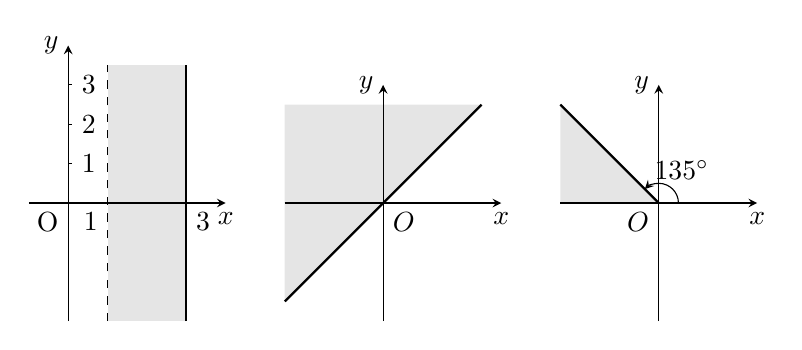
\begin{tikzpicture}[>=stealth, scale=.5]
\begin{scope}
    \fill[gray!20!white](1,-3) rectangle (3,3.5);
\draw[->](-1,0)--(4,0)node[below]{$x$};
\draw[->](0,-3)--(0,4)node[left]{$y$};
\foreach \x in {1,2,3}
{
    \draw(0,\x)--(.1,\x)node[right]{$\x$};
}

\draw[dashed](1,-3)--(1,3.5);
\draw[thick](3,-3)--(3,3.5);
\node[below left]{O};
\node at (1,0)[below left]{1};
\node at (3,0)[below right]{3};

\end{scope}
\begin{scope}[xshift=8cm]
    \fill[gray!20!white](-2.5,-2.5)--(-2.5,2.5)--(2.5,2.5)--cycle;
    \draw[->](-2.5,0)--(3,0)node[below]{$x$};
\draw[->](0,-3)--(0,3)node[left]{$y$};
\node[below right]{$O$};

\draw[thick](-2.5,-2.5)--(2.5,2.5);
\end{scope}
\begin{scope}[xshift=15cm]
    \fill[gray!20!white](-2.5,0)--(-2.5,2.5)--(0,0)--cycle;
    \draw[->](-2.5,0)--(2.5,0)node[below]{$x$};
\draw[->](0,-3)--(0,3)node[left]{$y$};
\node[below left]{$O$};
\draw[->](.5,0) arc (0:135:.5)node[above right]{$135^{\circ}$};
\draw[thick](-2.5,2.5)--(0,0);
\end{scope}
\end{tikzpicture}
    \caption*{第16题}
\end{figure}
\end{enumerate}



\subsection{复数的向量表示}
在物理学中,我们经常遇到力、速度、加速度、电场强度等,这些量,除了要考虑它们的绝对值的大小以外,还要考虑它们的方向,我们把这种既有绝对值大小又有方向的量叫做\textbf{向量}。向量可以用有向线段表示,线段的长度就是这个向量的绝对值(叫做这个\textbf{向量的模}),线段的方向(用箭头表示)就是这个向量的方向。模相等且方向相同的向量,不管它们的起点在哪里,都认为是\textbf{相等的向量}。在这一规定下,向量可以根据需要进行平移。模为零的向量(它的方向是任意的)叫做\textbf{零向量},规定所有的零向量相等。

\noindent
\begin{minipage}{.6\textwidth}\CTEXindent
复数可以用向量表示。前面我们已经看到
\[\text{复数集$\mathbb{C}$}\xleftrightarrow[]{\text{一一对应}}\text{复平面上的点集}\]
如图6.5中,复平面内点$Z(a,b)$表示复数$a+bi$,连接$OZ$,如果我们把有向线段$OZ$(方向是从原点$O$指向点$Z$)看成向量,记作$\VEC{OZ}$,这样就把复数同向量联系起来了。
\end{minipage}\hfill
\begin{minipage}{.35\textwidth}
\centering
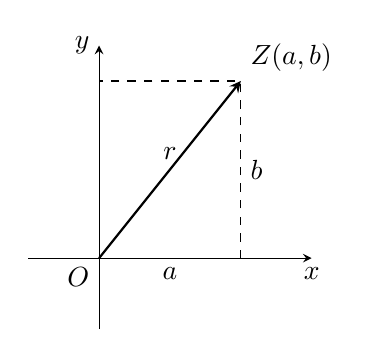
\begin{tikzpicture}[>=stealth, scale=.9]
    \draw[->](-1,0)--(3,0)node[below]{$x$};
    \draw[->](0,-1)--(0,3)node[left]{$y$};
    \node[below left]{$O$};
    \draw[dashed](2,0)--node[right]{$b$}(2,2.5)node[above right]{$Z(a,b)$}--(0,2.5);
\draw[->, thick](0,0)--node[above]{$r$}(2,2.5);
\node at (1,0)[below]{$a$};

\end{tikzpicture}   
\captionof{figure}{} 
\end{minipage}

很明显,从原点出发的向量$\VEC{OZ}$是由点$Z$所表示的复数唯一确定的;反过来,点$Z$所表示的复数也可以由从原点出发的向量$\VEC{OZ}$唯
一确定. 因此,复数集$\mathbb{C}$与复平面内所有以原点为起点的向量所成的集合也是一一对应的。此外,我们还规定,相等的向量表示同一个复数。

当$z=a+bi$用向量$\VEC{OZ}$表示时,
由于$\VEC{OZ}$的模(记作$|\VEC{OZ}|$)$r=\sqrt{a^2+b^2}$,于是,
我们也把$r$叫做\textbf{复数$a+bi$的模}(或\textbf{绝对值}),记作$|z|$或
$|a+bi|$. 因此有
\[|\VEC{OZ}|=|z|=|a+bi|=r=\sqrt{a^2+b^2}\]
其几何意义是复平面上表示复数$z$的点到原点的距离。

很有趣的是:当$b=0$时,$z=a+bi=a$, $|z|=|a|$,即$|z|$就是实数$a$的绝对值。可见,“复数的模(也叫复数的绝对值)”是实数的绝对值这一概念的扩充。

\begin{example}
    求复数$z_1=3+4i$与$z_2=-\frac{1}{2}-\sqrt{2}i$的模,并比较它们的大小(很明显,$|z|$是非负实数,所以可比大小).
\end{example}

\begin{solution}
\[\begin{split}
    |z_1|&=\sqrt{3^2+4^2}=5\\
|z_2|&=\sqrt{\left(-\frac{1}{2}\right)^2+\left(-\sqrt{2}\right)^2}=\sqrt{\frac{9}{4}}=\frac{3}{2}<5
\end{split}\]
$\therefore\quad |z_1|>|z_2|$.
\end{solution}

\noindent
\begin{minipage}{.5\textwidth}
    \begin{example}
    设$z\in\mathbb{C}$,且满足下列条件:
    \begin{enumerate}[(1)]
        \item $|z|=3$
        \item $2\le |z|<4$
    \end{enumerate}
试问在复平面上表示复数$z$的点集构成什么图形?
\end{example}
\end{minipage}\hfill
\begin{minipage}{.45\textwidth}
\centering
\begin{tikzpicture}[>=stealth]
\draw[dashed, pattern=north east lines](0,0) circle (1.6);
\draw[fill=white](0,0)node[below left]{$O$}circle (.8);
\node at (.8,0)[below left]{2};
\node at (1.6,0)[below right]{4};
\draw[->](-2,0)--(2.5,0)node[above]{$x$};
\draw[->](0,-2)--(0,2)node[left]{$y$};
\end{tikzpicture}
\captionof{figure}{}
\end{minipage}



\begin{solution}
\begin{enumerate}[(1)]
    \item 由$|z|=3$可知,表示复数$z$的点到原点的距离
    等于3,所以满足条件$|z|=3$的复数$z$的点集构成以原点为圆心,以3为半径的圆。
  \item 不等式$2\le |z|<4$可化为不等式组
    $\begin{cases}
        |z|<4\\ |z|\ge 2
    \end{cases}$

    不等式$|z|<4$的解集是圆$|z|=4$内部所有的点组成的集
    合,不等式$|z|\ge 2$的解集是圆$|z|=2$及其外部所有的点组成的集合,这两个集合的交集,就是上述不等式的解集,也就是满足条件$2\le |z|<4$的点$Z$的集合,即复数$z$所表示点的集合是以原点为圆心,半径分别为2与4的圆所夹的圆环,但不包括外圆的边界(图6.6)。
\end{enumerate}
\end{solution}


\begin{example}
    用复数表示下列复平面上的阴影区域(图6.7)。
\begin{figure}[htp]
    \centering
\begin{tikzpicture}[>=stealth]
\begin{scope}
    \draw(0,0)node[below left]{$O$} circle (1.6);
\node at (.8,0)[below left]{1};
\node at (1.6,0)[below right]{2};
\draw[->](-2,0)--(2.5,0)node[above]{$x$};
\draw[->](0,-2)node[below]{(1)}--(0,2)node[left]{$y$};
\draw[pattern=north east lines](-60:1.6)--(60:1.6)arc (60:-60:1.6);


\end{scope}
\begin{scope}[xshift=6cm]
    \draw(0,0) circle (1.6);
\node at (0,.8)[above right]{1};
\node at (0,-.8)[below right]{$-1$};
\draw[pattern=north east lines](-150:1.6)--(-30:1.6) arc (-30:30:1.6)--(150:1.6)arc (150:210:1.6);
\draw[fill=white](0,0)node[below left]{$O$}circle (.8);
\draw[->](-2,0)--(2.5,0)node[above]{$x$};
\draw[->](0,-2)node[below]{(2)}--(0,2)node[left]{$y$};
\end{scope}
\end{tikzpicture}
    \caption{}
\end{figure}
\end{example}

\begin{solution}
\begin{multicols}{2}
\begin{enumerate}[(1)]
    \item $\begin{cases}
        |z|\le 2\\ R(z)\ge 1
    \end{cases}$
    \item $\begin{cases}
        1\le |z|\le 2\\ -1\le I(z)\le 1
    \end{cases}$
\end{enumerate}
\end{multicols}
\end{solution}

\section*{习题二}
\begin{center}
\bfseries A
\end{center}

\begin{enumerate}
    \item 求证: \begin{enumerate}[(1)]
        \item 任给$z\in \mathbb{C}$, 都有$|z|=|\overline z|$
        \item 设$z\in \mathbb{C}$, 则$z=0\Longleftrightarrow|z|=0$
    \end{enumerate}
\item 比较$z_{1}=-5+12i$与$z_{2}=-6-6\sqrt{3}i$的模的大小。
\item 求证:复平面内分别和复数$z_1=1+2i$, $z_{2}=\sqrt{2}+\sqrt{3}i$, $z_{3}=\sqrt{3}-\sqrt{2}i$, $z_{4}=-2+i$
    对应的四点$Z_1,Z_2,Z_3,Z_4$共圆.
\item 若$|x+yi|=1\; (x,y\in \R)$, 求表示$z=x+yi$的点的轨
    迹。
\end{enumerate}


\begin{center}
    \bfseries B
    \end{center}

\begin{enumerate}\setcounter{enumi}{4}
   \item 设$z\in\mathbb{C}$,用阴影图示满足下列条件的复数在复平面上的
   点集。
\begin{multicols}{2}
\begin{enumerate}[(1)]
    \item   $|z| = 3$
    \item $|z| < 3$
    \item $ |z| > 3$
  \item  $ 2\leqslant | z| < 5$ 
  \item $ \big|| z| - 3\big| < 2$
   \item $\big||z|-2\big| +|z|-2=0$
\end{enumerate}    
\end{multicols}

 \item 设$z=x+yi\; (x,y\in \R)$, 满足下列条件的复数在复平面
   上的点集是什么图形?用阴影图示之。
\begin{multicols}{2}
\begin{enumerate}[(1)]
    \item  $0< | x| < 2$
    \item $x> 0,\quad y< 0,\quad x^{2}+ y^{2}< 16$
   \item    $y\geqslant 2$
\end{enumerate}
\end{multicols}
  
  \item  设$z\in\mathbb{C}$, 图示满足下列条件的点$z$的集合:
\begin{multicols}{2}
\begin{enumerate}[(1)]
    \item $|z|\leqslant3$, 且$R(z)\geqslant I(z)$
    \item $|z|=2$, 且$R(z)=-I(z)$
    \item $1\leqslant|z|<3$, 且$I(z)\leqslant-1$
\end{enumerate}
\end{multicols}

   \item 求出满足下列条件的复数$z$, 并且图示之。
\begin{multicols}{2}
\begin{enumerate}[(1)]
\item  $| z| = 1,\quad R( z) = -\frac 12$ 
\item  $| z| = 1,\quad R( z)= \frac 12$
\end{enumerate}
\end{multicols}
\end{enumerate}

\section{复数的四则运算}
在引言中我们已看到,当人们引入数$i$后,接踵而至的问题便是定义运算法则,并且希望这些新法则遵循“数集扩充的原则”。
(为书写简便,约定:本节中说到复数$a+bi$, $c+di$时,都假定$a,b,c,d\in\R$)

\subsection{复数的加法}
根据引言中提供的规定运算法则的原则,我们规定(定义)两复数$z_1=a+bi$, $z_2=c+di$的加法法则如下:
\begin{equation}
   (a+bi)+(c+di)=(a+c)+(b+d)i \tag{1}
\end{equation}
这就是说,$z_1,z_2$的和是个唯一确定的复数,它以$(a+c)$为实部,以$(b+d)$为虚部。

不难验证:
\begin{enumerate}
    \item 这样规定的加法法则满足交换律、结合律。即对任何$z_1,z_2,z_3\in\mathbb{C}$,都有
\[\begin{split}
    z_1+z_2&=z_2+z_1\\
(z_1+z_2)+z_3&=z_1+(z_2+z_3)    
\end{split}\]

\item 若$z_1,z_2\in\R$时,用这个法则与用实数加法 法则计算其和,结果是一致的。
\end{enumerate}

现在研究复数加法的几何意义。

从物理学知道,要求出作用于同一点$O$,但不在同一直线上的两个力$\VEC{F_1}$与$\VEC{F_2}$的合力,只要用表示$\VEC{F_1}$与$\VEC{F_2}$的向量为相邻的两边画一个平行四边形,那么,平行四边形中,以力
的作用点$O$为起点的那条对角线所表示的向量就是合力$\VEC{F}$[图6.8(1)]。这个法则通常叫做向量加法的平行四边形法则。

\begin{figure}[htp]
    \centering
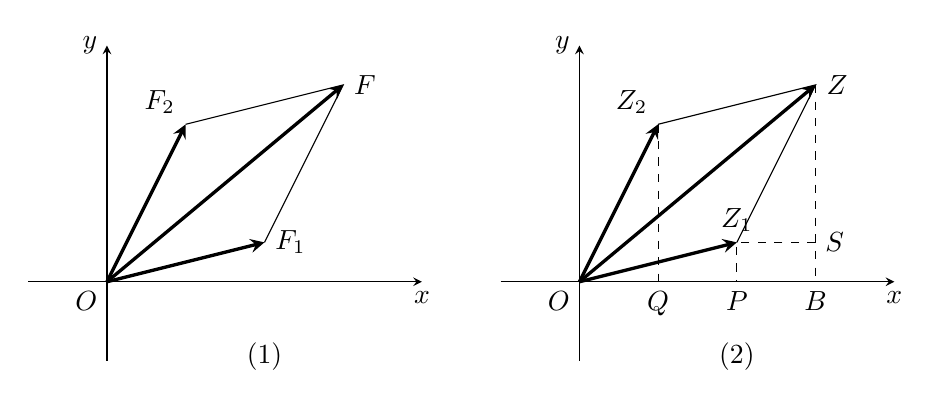
\begin{tikzpicture}[>=stealth]
\begin{scope}
    \draw[->](-1,0)--(4,0)node[below]{$x$};
    \draw[->](0,-1)--(0,3)node[left]{$y$};
\node[below left]{$O$};
\draw[->, very thick](0,0)--(1,2)node[above left]{$\vv{F_2}$};
\draw[->, very thick](0,0)--(2,.5)node[right]{$\vv{F_1}$};
\draw[->, very thick](0,0)--(3,2.5)node[right]{$\vv{F}$};
\draw(1,2)--(3,2.5)--(2,.5);
\node at (2,-.95){(1)};
\end{scope}
\begin{scope}[xshift=6cm]
    \draw[->](-1,0)--(4,0)node[below]{$x$};
    \draw[->](0,-1)--(0,3)node[left]{$y$};
\node[below left]{$O$};
\draw[->, very thick](0,0)--(1,2)node[above left]{$Z_2$};
\draw[->, very thick](0,0)--(2,.5)node[above]{$Z_1$};
\draw[->, very thick](0,0)--(3,2.5)node[right]{$Z$};
\draw(1,2)--(3,2.5)--(2,.5);
\draw[dashed](3,.5)node[right]{$S$}--(2,.5)--(2,0)node[below]{$P$};
\draw[dashed](1,2)--(1,0)node[below]{$Q$};
\draw[dashed](3,2.5)--(3,0)node[below]{$B$};
\node at (2,-.95){(2)};

\end{scope}
\end{tikzpicture}
    \caption{}
\end{figure}

复数用向量来表示,如果与这些复数对应的向量不在同一直线上,那么这些复数的加法就可以按照向量加法的平行四边形法则来进行。下面我们来证明这个事实。

设$\vv{OZ_1}$及$\vv{OZ_2}$分别与复数$a+bi$及$c+di$对应,且设$\vv{OZ_1}$, $\vv{OZ_2}$不在同一直线上[图6.8(2)]。以$\vv{OZ_1}$及$\vv{OZ_2}$为两条邻边画平行四边形$OOZ_1Z_2$,画$x$轴的垂线$PZ_1$, $QZ_2$及$RZ$,并且画$Z_1S\bot RZ$。容易证明
\[\triangle ZZ_1S\cong \triangle Z_2OQ\]
并且四边形$Z_1PRS$是矩形,因此
\[\begin{split}
 OR&=OP+PR=OP+Z_1S=OP+OQ=a+c\\
RZ&=RS+SZ=PZ_1+QZ_2=b+d
\end{split}\]

于是,点$Z$的坐标是$(a+c,b+d)$,这说明$\vv{OZ}$就是与复数$(a+c)+(b+d)i$对应的向量。

由此可知,求两个复数的和,可以先画出与这两个复数对应的向量$\vv{OZ_1}$, $\vv{OZ_2}$,如果$\vv{OZ_1}$, $\vv{OZ_2}$不在同一直线上,再以这两个向量为两条邻边画平行四边形,那么与这个平行四边形的对角线$OZ$所表示的向量$\vv{OZ}$对应的复数,就是所求两个复数的和。

如果$\vv{OZ_1}$, $\vv{OZ_2}$在同一直线上,我们可以画出一个“压扁”了的平行四边形,并据此画出它的对角线来表示$\vv{OZ_1}$, $\vv{OZ_2}$的和。

复数加法还可以用向量加法的三角形法则来进行。由图6.8(2)可以看出$\vv{OZ_2}$与$\vv{Z_1Z}$是相等的向量,因此可以平移向量$\vv{OZ_2}$,使其起点与向量$\vv{OZ_1}$的终点重合,得到向量$\vv{Z_1Z}$构成$\triangle OZ_1Z$,则向量$\vv{OZ}$就是所求两个复数的和。

\subsection{复数的减法}
复数的减法规定(定义)为复数加法的逆运算,即把满足
\begin{equation}
    (c+di)+(x+yi)=a+bi  \tag{2}
\end{equation}
的复数$x+yi$,叫做\textbf{复数$a+bi$减去复数$c+di$的差},记作$(a+bi)-(c+di)$.

根据复数相等的定义,由(2)得
\[\begin{cases}
    c+x=a\\d+y=b
\end{cases}\Longrightarrow \begin{cases}
    x=a-c\\y=b-d
\end{cases}\]
$\therefore\quad x+yi=(a-c)+(b-d)i$

从而
\[(a+bi)-(c+di)=(a-c)+(b-d)i\]
这就是复数的\textbf{减法法则}。由此可见,两复数的差也是一个唯一确定的复数。

由上所述,可以看出,复数的加(减)法与多项式的加(减)法是类似的,就是把复数的实部与实部、虚部与虚部分别相加(减)。

\begin{example}
    计算:
\begin{enumerate}[(1)]
\item $(-5+2i)+(7+4i)+(2-3i)$
\item $(5-6i)+(3-4i)-(2-5i)-(-7-4i)$
\end{enumerate}
\end{example}

\begin{solution}
\begin{enumerate}[(1)]
    \item $(-5+2i)+(7+4i)+(2-3i)=(-5+7+2)+(2+4-3)i=4+3i$
\item $(5-6i)+(3-4i)-(2-5i)-(-7-4i)=(5+3-2+7)+(-6-4+5+4)i=13-i$
\end{enumerate}
\end{solution}

\begin{example}
    设$z_1$、$z_2\in \mathbb{C}$, 求证:
$$\overline{z_{1}+z_{2}}=\overline{z_{1}}+\overline{z_{2}},\qquad\overline{z_{1}-z_{2}}=\overline{z_{1}}-\overline{z_{2}}$$
\end{example}

\begin{proof}
    设$z_1=a+bi,\quad z_2=c+di\; (a,b,c,d\in \R)$
\[\begin{split}
    \overline{z_{1}+z_{2}}&=\overline{(a+bi)+(c+di)}=\overline{(a+c)+(b+d)i}\\
    &=(a+c)-(b+d)i=(a-bi)+(c-di)\\
    &=\overline{z_{1}}+\overline{z_{2}}
\end{split}\]
(后一个证明,由读者完成)
\end{proof}

\begin{example}
    填空(设$z=a+bi,a,b\in \R$)
\[\begin{split}
    z+\overline{z}&=\blank\blank\\
    z-\overline{z}&=\blank\blank
\end{split}\]
\end{example}

现在研究复数减法的几何意义。

由于减法是加法的逆运算,从图6.8(2)中可以看出:如果向量$\vv{OZ}$表示复数$a+bi$,向量$\vv{OZ_1}$表示复数$c+di$,
则向量$\vv{OZ_2}$所表示的复数就是$(a+bi)-(c+di)$所得的差,而向量$\vv{Z_1Z}$与向量$\vv{OZ_2}$相等,因而它也表示$(a+bi)-(c+di)$所得的差。这就是说,在复平面上,连接表示两复数的点,方向指向被减复数,就能得到与两复数之差对应的向量,这就是复数减法的几何意义.

\begin{example}
    在复平面上,用复数表示两点间的距离公式。
\end{example}

\noindent
\begin{minipage}{.48\textwidth}
\CTEXindent
    \begin{solution}
    根据复数减法的几何意义,向量$\vv{Z_2Z_1}$表示两复数的差$z_1-z_2$(图6.9),由复数的模的定义可知
\[    |\vv{z_2z_1}|=|z_1-z_2|\]

又因为$|\vv{z_2z_1}|$就是复平面上两点$z_1$, $z_2$间的距离,我们把它记作$d$,就有
  \[  d=|z_1-z_2|\]

\end{solution}
\end{minipage}\hfill
\begin{minipage}{.5\textwidth}
\centering
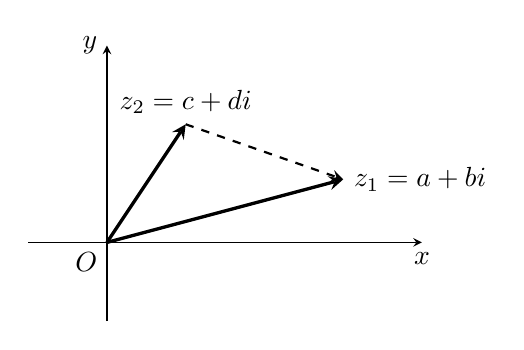
\begin{tikzpicture}[>=stealth]
    \draw[->](-1,0)--(4,0)node[below]{$x$};
    \draw[->](0,-1)--(0,2.5)node[left]{$y$};
\node[below left]{$O$};
\draw[very thick, ->](0,0)--(3,.8)node[right]{$z_1=a+bi$};
\draw[very thick, ->](0,0)--(1,1.5)node[above]{$z_2=c+di$};
\draw[thick, dashed, ->](1,1.5)--(3,.8);

\end{tikzpicture}
\captionof{figure}{}
\end{minipage}

  这就是复平面上表示复数$z_1$, $z_2$对应的两点间的\textbf{距离公式}.


\begin{example}
在复平面上,求表示下列每组复数对应的两点间的距离:
\begin{multicols}{2}
 \begin{enumerate}[(1)]
\item $z_1=3+2i,\quad z_2=-3-5i$
\item $z_3=a+bi,\quad z_4=c+di$
\end{enumerate}   
\end{multicols}
\end{example}

\begin{solution}
\begin{enumerate}[(1)]
    \item \[\begin{split}
        d_{z_1z_2}=|z_1-z_2|&=|(3+2i)-(-3-5i)|=|(3+5)+(2+5)i|\\
        &=|8+7i|=\sqrt{8^2+7^2}=\sqrt{113}\\
    \end{split}\]
    \item \[\begin{split}
        d_{z_3z_4}=|z_3-z_4|&=|(a+bi)-(c+di)|=|(a-c)+(b-d)i|\\
        &=\sqrt{(a-c)^2+(b-d)^2}\\
    \end{split}\]
\end{enumerate}
这与平面解析几何中两点间的距离公式是一致的.
\end{solution}

    \begin{example}
    在复平面上求圆的方程。
\end{example}

\noindent
\begin{minipage}{.55\textwidth}
\begin{solution}
设圆心对应的复数为$z_0=a+bi$,圆上任一点对应的复数为$z=x+yi$,圆的半径为$r$(图6.10),则根据圆的定义得
\[|z-z_0|=r\]
这就是复平面上圆的方程.
\end{solution}
\end{minipage}
\begin{minipage}{.45\textwidth}
    \centering
    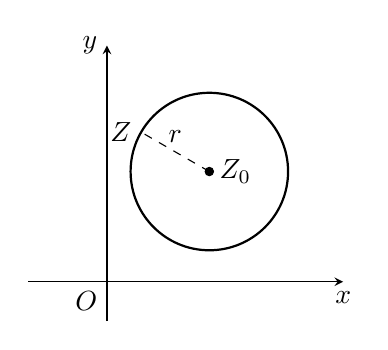
\begin{tikzpicture}[>=stealth]
        \draw[->](-1,0)--(3,0)node[below]{$x$};
        \draw[->](0,-.5)--(0,3)node[left]{$y$};
    \node[below left]{$O$};
    \draw[thick](1.3,1.4)node[right]{$Z_0$}circle (1);
    \draw[dashed](1.3,1.4)--node[above]{$r$}+(150:1)node[left]{$Z$};
    \draw[fill](1.3,1.4)circle(1.5pt);
    \end{tikzpicture}
    \captionof{figure}{}
\end{minipage}

应当明确,利用复数减法的几何意义和复数的模的定义所得出的复平面上两点间的距离公式是一个很重要的结果。与直角坐标平面上的两点间距离公式
\[d=\sqrt{(x_1-x_2)^2+(y_1-y_2)^2}\]
相比,它结构上更加简明、直接,因而对简化平面曲线的方程必将起到一定的作用。


\begin{example}
    若点$Z$满足$|z+2\sqrt{3}-2i|\le 1$,求$|z|$的最大值与最小值及相应的复数$z$。
\end{example}

\begin{solution}
    由于
\[|z+2\sqrt{3}-2i|=\left|z-\left(-2\sqrt{3}+2i\right)\right|\le 1\]

这一步先把条件写成$|z-z_0|$的形式,可知点$Z$的集合构成以$z_0=-2\sqrt{3}+2i$为圆心,以1为半径的一个圆面(图6.11),所以,使$|z|$最大(或最小)的点$Z$就是直线$OZ_0$与圆的两个交点$Z_1$和$Z_2$. 

\noindent
\begin{minipage}{.55\textwidth}
 \[\begin{split}
    |OZ_0|&=\sqrt{\left(-2\sqrt{3}\right)^2+2^2}=4\\
    |z|_{\max}&=|OZ_0|+R=4+1=5\\
    |z|_{\min}&=|OZ_0|-R=4-1=3\\
\end{split}\]
利用三角函数容易算出:
\[\begin{split}
    z_1&=-\frac{5}{2}\sqrt{3}+\frac{5}{2}i\\
    z_2&=-\frac{3}{2}\sqrt{3}+\frac{3}{2}i
\end{split} \]   
\end{minipage}\hfill
\begin{minipage}{.45\textwidth}
    \centering
    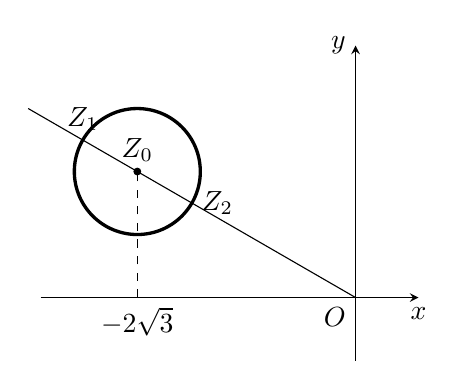
\begin{tikzpicture}[>=stealth, scale=.8]
        \draw[->](-5,0)--(1,0)node[below]{$x$};
        \draw[->](0,-1)--(0,4)node[left]{$y$};
    \node[below left]{$O$};
\draw[very thick](-2*1.732,2)circle(1);
    \draw[fill](-2*1.732,2)circle(1.5pt);
    \draw(0,0)--(-2*1.732,2)--(-3*1.732,3);
    \draw[dashed](-2*1.732,0)node[below]{$-2\sqrt{3}$}--(-2*1.732,2)node[above]{$Z_0$};
    \node at (150:3)[right]{$Z_2$};
    \node at (150:5)[above]{$Z_1$};
    \end{tikzpicture}
    \captionof{figure}{}
\end{minipage}
\end{solution}

\section*{习题三}
\begin{center}
    \bfseries A
\end{center}

\begin{enumerate}
    \item 证明复数加法满足交换律和结合律。
    \item 计算:
\begin{enumerate}[(1)]
\item $(2+3i)+(3-4i)+(4-8i)+(-2-6i)$
\item $\left(\frac{2}{3}+i\right)+\left(1-\frac{2}{3}i\right)-\left(\frac{1}{2}+\frac{3}{4}i\right)$
\item  $\left(-\sqrt{2}+\sqrt{3}i\right)-\left[\left(\sqrt{3}-\sqrt{2}\right)+\left(\sqrt{3}+\sqrt{2}i\right)\right]+\left(-\sqrt{2}i+\sqrt{3}\right)$
\item $[(a+b)+(a-b)i]-[(a-b)-(a+b)i]$
\item $(3-2i)-(-2+3i)+(5-4i)-(2-5i)-(-1+7i)$
\end{enumerate}

\item 在复平面上若$A$、$B$对应的复数是$6+5i$与$-3+4i$,
\begin{enumerate}[(1)]
 \item 求$\vv{OA}+\vv{OB}$表示的复数;
\item 求$\vv{AB}$表示的复数与$\vv{BA}$表示的复数;
\item 求$-\vv{OA}+\vv{OB}$表示的复数;
\item 求$(-\vv{OA})+(-\vv{OB})$表示的复数  
\end{enumerate}
\item 在复平面上,求表示下列各组复数对应的两点间的距离:
\begin{multicols}{2}
\begin{enumerate}[(1)]
\item $z_1=2+i,\quad z_2=3-i$
\item $z_3=8+5i,\quad z_4=4-2i$
\end{enumerate}
\end{multicols}

\item 复平面上两点对应的复数是$z_1,z_2$,以这两个点为端点的线段的垂直平分线的方程是\blank\blank
\item 复平面上一椭圆的两个焦点的坐标为$(-\sqrt{5},0)$和$(\sqrt{5},0)$,椭圆上的动点到两焦点的距离之和为6,椭圆的方程是\blank\blank
\end{enumerate}

\begin{center}
    \bfseries B
\end{center}

\begin{enumerate}\setcounter{enumi}{6}
\item 复平面上有两个定点,它们对应的复数是$z_1,z_2$,平面上动点到这两个定点距离之和为$2m$。当$2m>|z_1-z_2|$, $2m=|z_1-z_2|$, $2m<|z_1-z_2|$时,分别求动点的轨迹方程,并说明轨迹是什么图形。
\item 设$z_1,z_2$是非零复数,用几何方法证明著名的\textbf{三角形不等式}
\[\big||z_1|-|z_2| \big|\le |z_1\pm z_2|\le |z_1|+|z_2|\]
并指出等号成立的条件(注意分情况讨论)。
\item 复数$z$满足$|z+\sqrt{2}-\sqrt{2}i|\le 1$,求$|z|$的最大值与最小值,及相应的复数$z$。
\item 设$|z+1|=|z-i|$,且$z+2+\frac{4}{z+2}\in\R$,求$z$.
\end{enumerate}

\subsection{复数的乘法}
我们规定(定义)两个复数$z_1=a+bi$, $z_2=c+di$的乘法法则如下:
\[\begin{split}
   (a+bi)(c+di)&=ac+bci+adi+bdi^2\\
&=(ac-bd)+(bc+ad)i 
\end{split}\]
这就是说,复数的乘法能像多项式那样进行运算,但是必须把结果中的$i^2$换成$-1$,并将实部和虚部分别合并。由此可以看出,复数的积是唯一确定的一个复数。

容易验证,这样定义的乘法法则:
\begin{enumerate}[(1)]
\item 满足交换律、结合律和乘法对加法的分配律,即对任何$z_1,z_2,z_3\in\mathbb{C}$,有
\[\begin{split}
 z_1\cdot z_2&=z_2\cdot z_1\\
(z_1\cdot z_2)\cdot z_3&=z_1\cdot (z_2\cdot z_3)\\
z_1\cdot (z_2+z_3)&=z_1\cdot z_2+z_1\cdot z_3   
\end{split}\]

\item 正整数指数幂的运算律也能推广到复数集中,即对任何复数$z,z_1,z_2$,有
\[\begin{split}
    z^m\cdot z^n&=z^{m+n}\\
    (z^m)^n&=z^{m n}\qquad \qquad (m,n\in\N)\\
    (z_1\cdot z_2)^n&=z_1^n\cdot z_2^n
\end{split}\]
\item 若$z_1,z_2\in\R$时,用这个法则与用实数乘法法则计算其积,结果是一致的。
\end{enumerate}

有了如上的算律,现在研究$i^n=?$(其中$n\in\N$)
\[\begin{split}
    i^1&=i\\
    i^2&=-1\\
    i^3&=i^2\cdot i=-i\\
    i^4&=i^3\cdot i=(-i)\cdot i=1\\
\end{split}\]
从而,对于任何$n\in\N$,都有
\[\begin{split}
    i^{4n}&=(i^4)^n=1\\
    i^{4n+1}&=i^{4n}\cdot i=i\\
    i^{4n+2}&=i^{4n}\cdot i^2=-1\\
    i^{4n+3}&=i^{4n}\cdot i^3=-i\\
\end{split}\]

上述这些关系,称为虚数单位$i$乘方运算的\textbf{周期性}.


\begin{example}
    计算下列各式:
\begin{multicols}{2}
\begin{enumerate}[(1)]
    \item $i^{101}$ 
    \item $i^{9999}$ 
    \item $i+i^2+i^3+\cdots+i^{100}$ 
    \item $i^{n}+i^{n+1}+i^{n+2}+i^{n+3}\quad (n\in\N)$ 
\end{enumerate}
\end{multicols}
\end{example}

\begin{solution}
\begin{enumerate}[(1)]
    \item $i^{101}=i^{4\x 25+1}=i$ 
    \item $i^{9999}=i^{4\x 2499+3}=-i$ 
    \item $i+i^2+i^3+\cdots+i^{100}=\frac{i(1-i^{100})}{1-i}=\frac{i(1-i^{4\x 25})}{1-i}=\frac{i(1-1)}{1-i}=0$ 
    \item $i^{n}+i^{n+1}+i^{n+2}+i^{n+3}=i^n(1+i+i^2+i^3)=i^n(1+i-1-i)=0$ 
\end{enumerate}
\end{solution}

由(4)可以看出,虚数单位$i$的连续4个正整数次幂
的和为零,这是$i$的乘方运算的周期性造成的,也可以说是$i$的乘方运算周期性的另一种表现形式,利用这一结论,你能迅速简捷地计算出(3)式的结果吗?

现在计算很重要的$z\cdot \bar z=?$

设$z=a+bi\; (a,b\in\R)$,则
\[z\cdot \bar z=(a+bi)(a-bi)=a^2-(bi)^2=a^2+b^2\]
另一方面,
\[a^2+b^2=(\sqrt{a^2+b^2})^2=|z|^2=|\bar z|^2\]

比较以上两式,得到

\begin{thm}
{定理}对于任意的$z\in\mathbb{C}$,有
\[z\cdot \bar z=|z|^2=|\bar z|^2\]    
\end{thm}


应该注意:这个定理虽然形式上极其简单,但它却把$z$,$\bar z$,$|z|$,$|\bar z|$联系在一个等式之中,是一个非常重要的结果。

\begin{thm}
    {推论} 若$z$为虚数,则$|z|^2\ne z^2$.
(这与实数集上的结果是不同的!)
\end{thm}

\begin{example}
计算:
\begin{multicols}{2}
\begin{enumerate}[(1)]
    \item $(1-2i)(3+2i)(-1+3i)$
    \item $(-3+4i)(-3-4i)$
\end{enumerate}
\end{multicols}
\end{example}

\begin{solution}
\begin{enumerate}[(1)]
    \item $(1-2i)(3+2i)(-1+3i)=(7-4i)(-1+3i)=5+25i$
    \item $(-3+4i)(-3-4i)=(-3)^2-(4i)^2=25$
    
又解:$\text{原式}=(-3+4i)\overline{(-3+4i)}=|-3+4i|^2=(-3)^2+4^2=25$
\end{enumerate}

    
\end{solution}


\begin{example}
    计算$(x-1+i)(x-1-i)(x+1+i)(x+1-i),\quad (x\in\mathbb{R})$
\end{example}

\begin{solution}
\[\begin{split}
\text{原式}&=\left[(x-1)^{2}-i^{2}\right]\cdot \left[(x+1)^{2}-i^{2}\right]\\
&=(x^{2}-2x+1+1)(x^{2}+2x+1+1)\\
&=(x^{2}-2x+2)(x^{2}+2x+2)\\
&=(x^{2}+2)^{2}-(2x)^{2}\\
&=x^{4}+4x^{2}+4-4x^{2} =x^{4}+4
\end{split}\]
\end{solution}

\begin{remark}
由于复数的乘法能像多项式的乘法那样进行运算,所以在实数运算中的乘法公式都可以“移植”到复数中来,如在上例中我们就使用了平方差公式。
\end{remark}

\begin{example}
若$z_1,z_2\in\mathbb{C}$,证明下式,并解释它的几何意义:
\begin{equation}
  |z_1+z_2|^2+|z_1-z_2|^2=2|z_1|^2+2|z_2|^2  \tag{*}
\end{equation}
\end{example}

\begin{analyze}
式子中出现有“模的平方”,这就有可能利用$|z|^2=z\cdot \bar z$把(*)转化为易于运算的形式。
\end{analyze}

\begin{proof}
\[\begin{split}
    |z_1+z_2|^2+|z_1-z_2|^2&=(z_1+z_2)(\overline{z_1+z_2})+(z_1-z_2)(\overline{z_1-z_2})\\
&= (z_1+z_2)(\bar z_1+\bar z_2)+(z_1-z_2)(\bar z_1-\bar z_2)\\
&    =z_1\bar z_1+z_1\bar z_2+z_2\bar z_1+z_2\bar z_2+z_1\bar z_1-z_1\bar z_2-z_2\bar z_1+z_2\bar z_2\\
   & =|z_1|^2+|z_2|^2+|z_1|^2+|z_2|^2=2|z_1|^2+2|z_2|^2
\end{split}\]
\end{proof}    
    
\begin{analyze}
也可以设$z_1=a+bi,\; z_2=c+di\; (a,b,c,d\in\R)$去解。

    当表示$z_1,z_2$的点与原点不共线时,(*)表示平行四边形两对角线的平方和等于四条边的平方和(图6.12)。   
\end{analyze}

\begin{figure}[htp]
    \centering
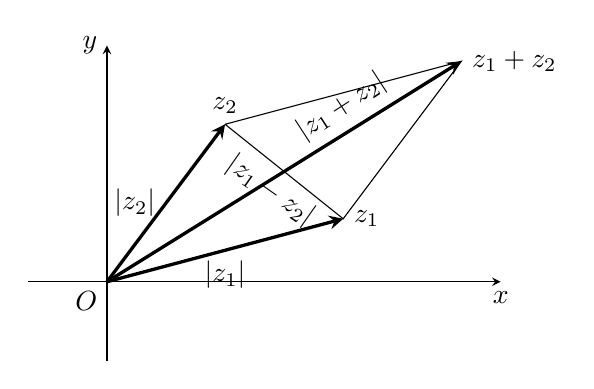
\begin{tikzpicture}[>=stealth]
    \draw[->](-1,0)--(5,0)node[below]{$x$};
    \draw[->](0,-1)--(0,3)node[left]{$y$};
\node[below left]{$O$};
\draw[very thick, ->](0,0)--node[left]{$|z_2|$}(1.5,2)node[above]{$z_2$};
\draw[very thick, ->](0,0)--node[below]{$|z_1|$}(3,.8)node[right]{$z_1$};
\draw[very thick, ->](0,0)--node[above, rotate=33, pos=.7]{$|z_1+z_2|$}(4.5,2.8)node[right]{$z_1+z_2$};
\draw(1.5,2)--(4.5,2.8)--(3,.8)--node[below, rotate=-35]{$|z_1-z_2|$}(1.5,2);
\end{tikzpicture}
    \caption{}
\end{figure}

\begin{remark}
\begin{enumerate}[(1)]
    \item  此例与例6.14(2)中展示的应用公式$z\cdot \bar z=|z|^2$的两种方式应掌握;
    \item 当$O,z_1,z_2$表示的点不共线时,应充分认识$|z_1|,|z_2|,|z_1+z_2|$能构成三角形, $|z_1|,|z_2|,|z_1-z_2|$也能构成三角形,从而得到利用几何方法解决复数问题的渠道.
\end{enumerate}
\end{remark}

\section*{习题四}
\begin{center}
    \bfseries A
\end{center}

\begin{enumerate}
    \item 证明复数的乘法满足交换律、结合律以及乘法对加法的分配律。
    \item  计算:
\begin{multicols}{2}
\begin{enumerate}[(1)]
    \item $(-8-7i)(-3i)$
    \item $(4-3i)(-5-4i)$
    \item $\left(-\frac{1}{2}+\frac{\sqrt{3}}{2}i\right)(1+i)$
    \item $\left(\frac{\sqrt{3}}{2}i-\frac{1}{2}\right)\left(-\frac{1}{2}+\frac{\sqrt{3}}{2}i\right)$
\end{enumerate}    
\end{multicols}

\item (口答)$i^{11},\; i^{25},\; i^{26},\; i^{70},\; i^{100},\; i^{400},\; i^{1000},\; i^{1002}$各等于什么?

\item 计算:
\begin{enumerate}[(1)]
\item $(-0.2+0.3i)(0.5-0.4i)$
\item $(1-2i)(2+i)(3-4i)$
\item $(\sqrt{a}+\sqrt{b}i)(\sqrt{a}-\sqrt{b}i)\quad (a,b\in\R^+)$
\item $(a+bi)(a-bi)(-a+bi)(-a-bi)$
\item $(a+bi)(a^2-abi-b^2)$
\item $(a-bi)(a^2+abi-b^2)$
\end{enumerate}

\item 
利用公式$a^2+b^2=(a+bi)(a-bi)$,把下列各式分解成一次因式的积:
\begin{multicols}{2}
\begin{enumerate}[(1)]
\item $x^2+4$
\item $a^4-b^4$
\item $a^2+2ab+b^2+c^2$
\item $x^2+2x+3$
\end{enumerate}
\end{multicols}

\item 计算$(1-i)+(2-i^3)+(3-i^5)+(4-i^7)$
\item 填空(并记住这些结果):
\begin{enumerate}
    \item $(1+i)^2=\blank\blank$
    \item $(1-i)^2=\blank\blank$
    \item $i^{4n+1}\cdot i^{4n+2}\cdot i^{4n+3}\cdot i^{4n+4} =\blank\blank$ (其中$n\in\N$或$n=0$)
\end{enumerate}
\item 计算:
\begin{multicols}{2}
\begin{enumerate}[(1)]
    \item $(1+i)^{10}$
    \item $(1-i)^6$
    \item $\left(-\frac{1}{2}+\frac{\sqrt{3}}{2}i\right)^7$
\end{enumerate}
\end{multicols}
\end{enumerate}

\begin{center}
    \bfseries B
\end{center}

\begin{enumerate}\setcounter{enumi}{8}
    \item 求证:若$z_1,z_2\in\mathbb{C}$,且$z_1\cdot z_2=0$,则中至少有一个是零。
    (提示:从复数$z$为0的定义入手)
    \item 设$z_1,z_2\in\mathbb{C}$, 满足$|z_1|=|z_2|=1$,且$|z_1+z_2|=\sqrt{2}$, 求$|z_1-z_2|$.
    \item 复平面内,一个平行四边形的三个顶点分别表示复数
    $0,\; 4+7i,\; -2+9i$,求第四个顶点表示的复数。
\end{enumerate}

\subsection{复数的除法}

复数的除法规定(定义)为乘法的逆运算,即把满足
\begin{equation}
  (c+di)(x+yi)=a+bi\quad (c+di\ne 0)  \tag{3}
\end{equation}
的复数$x+yi$,叫做复数$a+bi$除以$c+di$的商,记作$(a+bi)\div (c+di)$或$\frac{a+bi}{c+di}$. 现在,利用(3)式,求出$x+yi$.

由于$c+di\ne 0$,所以,在(3)式两边分别乘以$\overline{c+di}=c-di$,有
\[(c-di)(c+di)(x+yi)=(a+bi)(c-di)\]
即$(c^2+d^2)x+(c^2+d^2)yi=(ac+bd)+(bc-ad)i$,
利用复数相等的定义,得
\[x=\frac{ac+bd}{c^2+d^2},\qquad y=\frac{bc-ad}{c^2+d^2}\]
$\therefore\quad (a+bi)\div (c+di)=x+yi=\frac{ac+bd}{c^2+d^2}+\frac{bc-ad}{c^2+d^2}i$ \hfill(4)

另一方面,若把$(a+bi)\div (c+di)$形式地写作
\begin{equation}
 \frac{a+bi}{c+di}=\frac{(a+bi)\cdot (c-di)}{(c+di)\cdot (c-di)}\xRightarrow[]{\text{分离实虚部}}\frac{ac+bd}{c^2+d^2}+\frac{bc-ad}{c^2+d^2}i  \tag{5}
\end{equation}

比较(4),(5)可见,欲求两复数的商,可先写成“分式”,然后使分母“实数化”,再把实部与虚部分离即
\[\begin{split}
    (a+bi)\div (c+di)=\frac{a+bi}{c+di}&=\frac{(a+bi) (c-di)}{(c+di) (c-di)}\\
    &=\frac{ac+bd}{c^2+d^2}+\frac{bc-ad}{c^2+d^2}i
\end{split}\]

\begin{example}
计算$(1+2i)\div (3-4i)$
\end{example}

\begin{solution}
\[\begin{split}
    (1+2i)\div (3-4i)=\frac{1+2i}{3-4i}&=\frac{(1+2i)\cdot (3+4i)}{(3-4i)\cdot (3+4i)}\\
    &=\frac{-5+10i}{3^2+4^2}=-\frac{1}{5}+\frac{2}{5}i
\end{split}\]
\end{solution}


\begin{example}
    解方程$(5z-1)i+3z-2i=0$,其中$z\in\mathbb{C}$.
\end{example}

\begin{solution}
\textbf{解1:}设$z=x+yi\; (x,y\in\R)$,则有
\[(5x+5yi-1)i+3x+3yi-2i=0\]
即:$(3x-5y)+(5x+3y-3)i=0$

由于$x,y\in\R$,利用复数相等的定义,得
\[\begin{cases}
    3x-5y=0\\ 5x+3y-3=0
\end{cases}\]
解之,得:$x=\frac{15}{34},\quad y=\frac{9}{34}$

$\therefore\quad z=\frac{15}{34}+\frac{9}{34}i$

\textbf{解2:}原方程同解于$(5i+3)z=3i$,根据复数除法的定义,$z$是$3i$除以$(3+5i)$的商,即
\[z=\frac{3i}{3+5i}=\frac{3i\cdot (3-5i)}{(3+5i)\cdot (3-5i)}=\frac{15+9i}{3^2+5^2}=\frac{15}{34}+\frac{9}{34}i\]
\end{solution}

\begin{rmk}
与解1相比,解2简明得多。其步骤与解实系数一元一次方程相似,但应着重理解这里使用了复数除法的定义.
\end{rmk}

\begin{example}
    若$z_1,z_2\in\mathbb{C}$,求证
\begin{multicols}{2}
    \begin{enumerate}[(1)]
        \item $\overline{z_1\cdot z_2}=\overline{z_1}\cdot \overline{z_2}$
        \item $\overline{\left(\frac{z_1}{z_2}\right)}=\frac{\overline{z_1}}{\overline{z_2}}\quad (z_2\ne 0)$
    \end{enumerate}
\end{multicols}
\end{example}

\begin{analyze}
由共轭复数的概念,要解决此问题必须分清复数的实部与虚部,为此可设$z_1=a+bi,\; z_2=c+di\quad (a,b,c,d\in\R)$.
\end{analyze}

\begin{proof}
\begin{enumerate}[(1)]
    \item 设$z_1=a+bi,\; z_2=c+di\quad (a,b,c,d\in\R)$,
\[\begin{split}
    \because\quad \overline{z_1\cdot z_2}=\overline{(a+bi)\cdot (c+di)}
    &=\overline{(ac-bd)+(ad+bc)i}\\
    &=(ac-bd)-(ad+bc)i\\
    \overline{z_1}\cdot \overline{z_2}=\overline{a+bi}\cdot \overline{c+di}
    &=(a-bi)\cdot (c-di)\\
    &=(ac-bd)-(ad+bc)i\\
\end{split}\]
$\therefore\quad \overline{z_1\cdot z_2}=\overline{z_1}\cdot \overline{z_2}$

\item 由读者自己完成证明.
\end{enumerate}    
\end{proof}

\section*{习题五}
\begin{center}
    \bfseries A
\end{center}

\begin{enumerate}
    \item (口答)$\frac{1}{i},\; \frac{1}{i^3},\; \frac{1}{\sqrt{2}i},\; \left(\frac{1}{i}\right)^5,\; \frac{1+i}{1-i}$各等于什么?
    \item 计算: 
\begin{multicols}{2}
    \begin{enumerate}[(1)]
        \item $\frac{1}{11-5i}$
        \item $\frac{7-9i}{1+i}$
        \item $\frac{1-2i}{3+4i}$
        \item $\frac{1+2i}{2+4i}$
        \item $\frac{(1-2i)^2}{3-4i}-\frac{(2+i)^2}{4-3i}$
        \item $\frac{\sqrt{5}+\sqrt{3}i}{\sqrt{5}-\sqrt{3}i}-\frac{\sqrt{3}+\sqrt{5}i}{\sqrt{3}-\sqrt{5}i}$
    \end{enumerate}
\end{multicols}
    \item 计算: 
\begin{multicols}{2}
    \begin{enumerate}[(1)]
        \item $\left(\frac{1+i}{1-i}\right)^{10}$
        \item $(3+3i)^4$
        \item $\left(\frac{2+2i}{5-5i}\right)^4$
        \item $(a+ai)^6$
    \end{enumerate}
\end{multicols}
\item 设$f(z)=\frac{z^2-z+1}{z^2+z+1}$,求:
\begin{multicols}{2}
    \begin{enumerate}[(1)]
        \item $f(2+3i)$
        \item $f(2-3i)$
        \item $f(1-i)$
        \item $f(1+i)$
    \end{enumerate}
\end{multicols}
\end{enumerate}

\begin{center}
    \bfseries B
\end{center}

\begin{enumerate}\setcounter{enumi}{4}
    \item 已 知$z_{1}= 5+ 10i,\quad z_{2}= 3- 4i,\quad \frac 1z= \frac 1{z_{1}}+ \frac 1{z_{2}}$, 求$z$.
    \item 已知复数$z$的平方等于$5-12i$, 求$z$.
    \item 设$z\in \mathbb{C}$, 解方程:
\begin{multicols}{2}
\begin{enumerate}[(1)]
    \item $\frac 12 ( z- 1) = \frac {\sqrt {3}}2 ( 1+ z) i$
    \item $(z-i)i=3(z-3)$ 
\end{enumerate}
\end{multicols}

\item 设$x,y\in \mathbb{C}$, 解方程组
    $\begin{cases}
        (3+i)x+(3-i)y=16 \\
        (3+2i)x+(3-2i)y=14
    \end{cases}$
\item 设$x,y,z\in \mathbb{C}$, 解方程组
    $\begin{cases}
        x+iy-2z=10\\
        x-y+2iz=20\\
        ix+3iy-(1+i)z=30
    \end{cases}$
\item 定义$i^0$的意义是1,$i^-m$ 的意义是$\frac1{i^m}\; (m\in \N)$, 求证
\begin{enumerate}[(1)]
\item $i^{4n+ 1}= i$, $i^{4n+ 2}= - 1$, $i^{4n+ 3}= - i$, $i^{4n+ 4}= 1$
    对一切$n\in \Z$都成立(这个命题说明了什么)。
\item 证明$i^m+i^{m+1}+i^{m+2}+i^{m+3}=0$(其中$m\in \Z$).
\end{enumerate}
    
\item 若$(x+yi)^3=a+bi,\; (a,b,x,y\in \R)$, 求证
    $$\frac ax+\frac by=4(x^2-y^2)$$
\item $z=a+bi\; (a,b\in \R)$是关于$x$的实系数方程
    $$f(x)=mx^3+nx^2+px+q=0\quad (m\neq0)$$
    的一个根。求证:$\bar{z}=a-bi$也是此方程的根。

\end{enumerate}

\section{复数的三角形式}
复数的三角形式是彻底解决复数乘、除、乘方和开方题的桥梁。因此确定复数的三角形式是很重要的。

\subsection{复数的模与辐角}

前面我们已经学过,复数$z=a+bi$可以用复平面上的点表示(图6.13),进而,又可以用从原点出发的向量$\vv{OZ}$表
示。由此容易想到,复数是否也可以用$r$与$\theta$表示呢?

\begin{figure}[htp]
    \centering
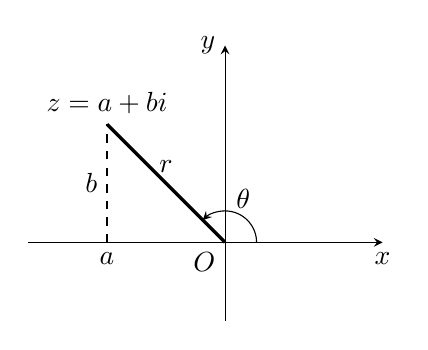
\begin{tikzpicture}[>=stealth]
\draw[->](-2.5,0)--(2,0)node[below]{$x$};
\draw[->](0,-1)--(0,2.5)node[left]{$y$};
\draw[->](.4,0) arc (0:135:.4);
\node at (135/2:.6){$\theta$};
\draw[very thick](0,0)--node[above]{$r$}(-1.5,1.5)node[above]{$z=a+bi$};
\draw[dashed](-1.5,0)node[below]{$a$}--node[left]{$b$}(-1.5,1.5);
\node[below left]{$O$};
\end{tikzpicture}
    \caption{}
\end{figure}

\begin{enumerate}
    \item 当$z\ne 0$时,$r=|\vv{OZ}|=\sqrt{a^2+b^2}$,称为$z$的\textbf{模},显然$z$有唯一的
    模,$\theta$是$\vv{OX}$转到$\vv{OZ}$的角,称为复数$z$的\textbf{辐角}\footnote{arg是英语单词argument(辐角)的前三个字母.},记为
 \[   {\rm Arg\,} z=\theta\]

    很明显,${\rm Arg\,}z$是多值的。事实上,若$z$的一个辐角是$\alpha$,则有${\rm Arg\,}z=\alpha+2k\pi\; (k\in\Z)$. 如复数$i$的辐角${\rm Arg\,}i=\frac{\pi}{2}+2k\pi\; (k\in\Z)$.

    为了今后使用上方便,把属于$[0,2\pi)$的$z$的辐角叫做$z$的辐角的\textbf{主值},记作$\arg z$,即
    \[0\le \arg z<2\pi\]

    由此可以看出,非零复数$z$有唯一的$\arg z$,而且
\begin{equation}
     {\rm Arg\,}z=\arg z+2k\pi\quad (k\in\Z)\tag{1}
\end{equation}
    \item 当$z=0$时,$|z|=0$,规定任意一个周内角都可以作为$z$的辐角的主值。
\end{enumerate}

\begin{ex}
\begin{enumerate}
\item   (填空):若$m\in\R^+$,则
\begin{multicols}{2}
\begin{enumerate}[(1)]
    \item $\arg m=\blank\blank$
    \item $\arg(-m)=\blank\blank$
    \item $\arg(mi)=\blank\blank$
    \item $\arg(-mi)=\blank\blank$
\end{enumerate}
\end{multicols}


\item 判断下列命题的真假:
\begin{enumerate}[(1)]
\item 每个复数对应唯一确定的模\hfill
(\quad)
\item 每个复数对应唯一确定的辐角的主值\hfill
(\quad)
\item 两个非零复数相等$\Leftrightarrow$它们的模与辐角的主值分别相等\hfill
(\quad)
\end{enumerate}

\end{enumerate}

\end{ex}


\subsection{用模与辐角表示复数}

从三角函数定义我们知道(图6.13):
\[\begin{cases}
    \frac{a}{r}=\cos \theta\\
    \frac{b}{r}=\sin\theta
\end{cases}\Rightarrow \begin{cases}
    a=r\cos\theta\\
    b=r\sin\theta
\end{cases}\]
\[z=a+bi=r\cos\theta+ir\sin\theta\]
\begin{equation}
  z=r(\cos\theta+i\sin\theta)\tag{2}
\end{equation}
(2)称为复数$z$的\textbf{三角形式}。为了区别,把$a+bi\; (a,b\in\R)$称作$z$的\textbf{代数形式}.

\begin{example}
    把下列复数表示成三角形式:
\begin{multicols}{3}
\begin{enumerate}[(1)]
    \item $z_1=\sqrt{3}+i$
    \item $z_2=1-i$
    \item $z_3=-1$
\end{enumerate}
\end{multicols}
\end{example}

\begin{analyze}
    欲化成三角形式,关键是求出$r$、$\theta$,这只要在复平面上先确定点$z$的位置就好办了.
\end{analyze}

\begin{solution}
\begin{enumerate}[(1)]
    \item $\because\quad r_1=\sqrt{\left(\sqrt{3}\right)^2+1}=2,\quad \theta_1=\frac{\pi}{6}$ (图6.14)

$\therefore\quad z_1=2\left(\cos\frac{\pi}{6}+i\sin\frac{\pi}{6}\right)$

\item $\because\quad r_2=\sqrt{2},\quad \theta_2=-\frac{\pi}{4}$ (图6.15)

$\therefore\quad z_2=\sqrt{2}\left[\pcx{-\frac{\pi}{4}}\right]$

\noindent
\begin{minipage}{.3\textwidth}
\centering
\begin{tikzpicture}[>=stealth]
    \draw[->](-1,0)--(2,0)node[right]{$x$};
    \draw[->](0,-1)--(0,2)node[left]{$y$};
\draw[very thick](0,0)node[below left]{$O$}--(1.732,1)node[above]{$z_1=\sqrt{3}+i$};
\draw[dashed](1.732,0)--node[right]{1}(1.732,1);
\node at (1.732/2,0)[below]{$\sqrt{3}$};
\draw[->](.5,0)arc (0:30:.5)node[right=.25]{$\tfrac{\pi}{6}$};
\draw[fill=white](1.732,1) circle(1.5pt);
\end{tikzpicture}
\captionof{figure}{}
\end{minipage}\hfill
\begin{minipage}{.3\textwidth}
    \centering
\begin{tikzpicture}[>=stealth]
    \draw[->](-1,0)--(2,0)node[right]{$x$};
    \draw[->](0,-2)--(0,1)node[left]{$y$};
\draw[very thick](0,0)node[below left]{$O$}--(1,-1)node[below]{$z_2=1-i$};
\draw[dashed](1,0)node[above]{1}--(1,-1);
\draw[->](.5,0)arc (0:-45:.5)node[right=.14]{$-\tfrac{\pi}{4}$};
\draw[fill=white](1,-1) circle(1.5pt);   
\end{tikzpicture}
\captionof{figure}{}
\end{minipage}\hfill
\begin{minipage}{.3\textwidth}
    \centering
\begin{tikzpicture}[>=stealth]
    \draw[->](-1.5,0)--(1.5,0)node[right]{$x$};
    \draw[->](0,-1)--(0,2)node[left]{$y$};
\node[below left]{$O$};
\draw[->](.5,0)arc (0:180:.5);
\draw[fill=white](-1,0)node[below]{$-1$} circle(1.5pt);
\node at (-1,0)[above]{$Z_3$};
\node at (120:.5)[above]{$\pi$};
\end{tikzpicture}
\captionof{figure}{}
\end{minipage}

\item $\because\quad r_3=1,\quad \theta_3=\pi$ (图6.16)

$\therefore\quad z_3=\pc{\pi}$
\end{enumerate}
\end{solution}

\begin{example}
判断下列各式是否是三角形式,若不是,化为三角形式:
\begin{multicols}{2}
\begin{enumerate}[(1)]
    \item $z_1=-2\left(\pc{\frac{\pi}{3}}\right)$
    \item $z_2=2(\cos\theta-i\sin\theta)$
    \item $z_3=3(\sin\theta+i\cos\theta)$
    \item $z_4=-2(\sin\theta+i\cos\theta)$
    \item $z_5=2(\cos90^{\circ}+i\sin30^{\circ})$
\end{enumerate}
\end{multicols}
\end{example}

\begin{solution}
\begin{enumerate}[(1)]
    \item 这不是三角形式。
    
    容易看出在复平面上$z_1$是$z_0=2\left(\pc{\frac{\pi}{3}}\right)$关于原点的对称点(图6.17),从而
\[z_1=2\left[\pcx{\frac{\pi}{3}+\pi}\right]=2\left(\pc{\frac{4\pi}{3}}\right)\]

\noindent
\begin{minipage}{.45\textwidth}
    \centering
\begin{tikzpicture}[>=stealth]
    \draw[->](-2,0)--(2,0)node[right]{$x$};
    \draw[->](0,-2)--(0,2)node[left]{$y$};
\draw[very thick](-1,-1.732)node[below]{$Z_1$}--(0,0)node[below right]{$O$}--(1,1.732)node[above]{$Z_0$};
\draw[->](.5,0)arc (0:60:.5)node[right=.1]{$\frac{\pi}{3}$};
\draw[fill=white](-1,-1.732) circle(1.5pt);   
\draw[fill=white](1,1.732) circle(1.5pt);   
\end{tikzpicture}
\captionof{figure}{}
\end{minipage}\hfill
\begin{minipage}{.45\textwidth}
    \centering
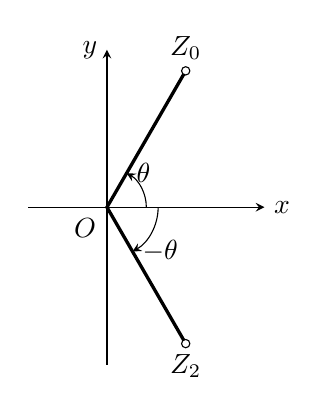
\begin{tikzpicture}[>=stealth]
    \draw[->](-1,0)--(2,0)node[right]{$x$};
    \draw[->](0,-2)--(0,2)node[left]{$y$};
\draw[very thick](1,-1.732)node[below]{$Z_2$}--(0,0)node[below left]{$O$}--(1,1.732)node[above]{$Z_0$};
\draw[->](.5,0)arc (0:60:.5)node[right=.1]{$\theta$};
\draw[fill=white](1,-1.732) circle(1.5pt);   
\draw[fill=white](1,1.732) circle(1.5pt);   
\draw[->](.65,0)arc (0:-60:.65)node[right=.1]{$-\theta$};

\end{tikzpicture}
\captionof{figure}{}
\end{minipage}


\item 这也不是三角形式。在复平面上,视$\theta$为锐角时$z_2$是$z_0=2(\cos\theta+i\sin\theta)$关于实轴的对称点(图6.18),从而
\[z_2=2[\cos(-\theta)+i\sin(-\theta)]\]

\item  这也不是三角形式。从图6.19可以看出,$z_3$的辐角是$\frac{\pi}{2}-\theta$.

$\therefore\quad z_3=3\left[\pcx{\frac{\pi}{2}+\theta}\right]$

\item 这也不是三角形式。从图6.20可以看出$z_4$是$z_0$关于原点的对称点。$z_0$的辐角是$\frac{\pi}{2}-\theta$,从而$z_4$的辐角是$\frac{3\pi}{2}-\theta$.

$\therefore\quad z_4=2\left[\pcx{\frac{3\pi}{2}-\theta}\right]$

\noindent
\begin{minipage}{.45\textwidth}
    \centering
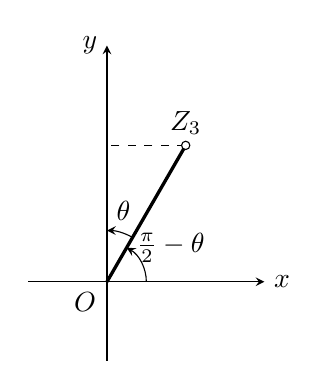
\begin{tikzpicture}[>=stealth]
      \draw[->](-1,0)--(2,0)node[right]{$x$};
    \draw[->](0,-1)--(0,3)node[left]{$y$};
\draw[very thick](0,0)node[below left]{$O$}--(1,1.732)node[above]{$Z_3$};
\draw[->](.5,0)arc (0:60:.5)node[right=.1]{$\frac{\pi}{2}-\theta$};
\draw[dashed](1,1.732)--(0,1.732);
\draw[fill=white](1,1.732) circle(1.5pt);   
\draw[->](60:.65)arc (60:90:.65)node[above right]{$\theta$};

\end{tikzpicture}
\captionof{figure}{}
\end{minipage}\hfill
\begin{minipage}{.45\textwidth}
    \centering
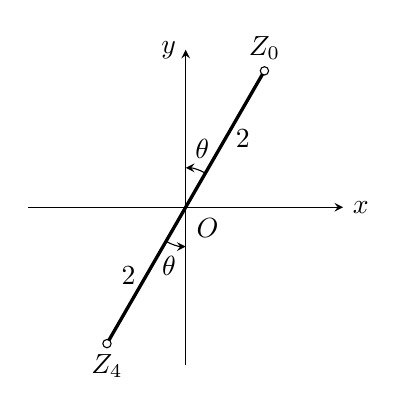
\begin{tikzpicture}[>=stealth]
    \draw[->](-2,0)--(2,0)node[right]{$x$};
    \draw[->](0,-2)--(0,2)node[left]{$y$};
\draw[very thick](-1,-1.732)node[below]{$Z_4$}--node[left]{2}(0,0)node[below right]{$O$}--node[right]{2}(1,1.732)node[above]{$Z_0$};
\draw[->](60:.5)arc (60:90:.5)node[above right]{$\theta$};
\draw[->](240:.5)arc (240:270:.5)node[below left]{$\theta$};
\draw[fill=white](-1,-1.732) circle(1.5pt);   
\draw[fill=white](1,1.732) circle(1.5pt); 
\end{tikzpicture}
\captionof{figure}{}
\end{minipage}    

\item 这也不是三角形式。
\[z_5=2(\cos90^{\circ}+i\sin30^{\circ})=i=\pc{\frac{\pi}{2}}\]
\end{enumerate}    
\end{solution}

\begin{rmk}
    解决这类问题必须:
\begin{enumerate}[(1)]
\item 对复数三角形式的结构特征要理解得很清楚,其中$r\ge \theta$;前面是$\theta$角的余弦,后面是$\theta$角的正弦;中间用加号连接。
\item 上面的方法是:把$\theta$ 视为锐角,先在第一象限中构造出与$z$对称的点$z_0$,再根据符号画出点$z$,最后利用$z$与$z_0$的对称性写出$z$的模与辐角。
\item 也可以直接使用诱导公式解决问题:把$\theta$ 视为锐角后,由符号定$z$所在象限,再看函数变不变,以确定用哪个诱导公式。如对$z_4$,由符号定出它在第三象限,且两个弦
函数名称都需要变,从而用$\frac{3\pi}{2}-\theta$的诱导公式就行了.   

$\therefore\quad z_4=2\left[\pcx{\frac{3\pi}{2}-\theta}\right]$
\end{enumerate}
\end{rmk}

\begin{example}
化下列复数为三角形式:
\begin{multicols}{2}
\begin{enumerate}[(1)]
    \item $z_1=-4+3i$
    \item $z_2=5-12i$
\end{enumerate}
\end{multicols}
\end{example}

\begin{solution}
\begin{enumerate}[(1)]
    \item 先在第一象限构造$z_1$的对称点$z_0=4+3i$,立刻有

$|z_0|=\sqrt{4^2+3^2}=5,\qquad \arg z_0=\arctan\frac{3}{4}$\hfill (图6.21)

$\therefore\quad z_1=5\left[\pcx{\pi-\arctan\frac{3}{4}}\right]$

\begin{figure}[htp]
    \centering
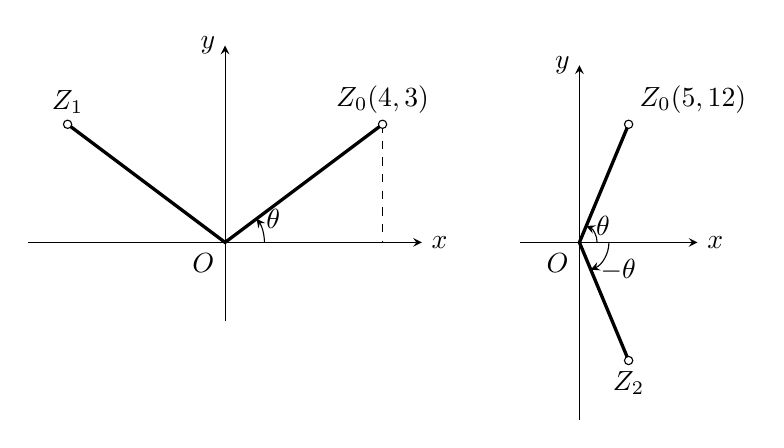
\begin{tikzpicture}[>=stealth, scale=.5]
\begin{scope}
    \draw[->](-5,0)--(5,0)node[right]{$x$};
    \draw[->](0,-2)--(0,5)node[left]{$y$};
\draw[very thick](-4,3)node[above]{$Z_1$}--(0,0)node[below left]{$O$}--(4,3)node[above]{$Z_0(4,3)$};
\draw[->](1,0)arc(0:36.87:1)node[right]{$\theta$};

\draw[dashed](4,3)--(4,0);
\draw[fill=white](4,3) circle(3pt);
\draw[fill=white](-4,3) circle(3pt);
\end{scope}
\begin{scope}[xshift=9cm, scale=1.5]
    \draw[->](-1,0)--(2,0)node[right]{$x$};
    \draw[->](0,-3)--(0,3)node[left]{$y$};
\draw[very thick](5/6,-2)node[below]{$Z_2$}--(0,0)node[below left]{$O$}--(5/6,2)node[above right]{$Z_0(5,12)$};
\draw[->](.3,0)arc(0:67.38:.3)node[right]{$\theta$};
\draw[->](.5,0)arc(0:-67.38:.5)node[right]{$-\theta$};

\draw[fill=white](5/6,2) circle(2pt);
\draw[fill=white](5/6,-2) circle(2pt);
\end{scope}
\end{tikzpicture}
    \caption{}
\end{figure}


\item 在第一象限构造$z_2$的对称点$z_0=5+12i$,则
\[|z_0|=13,\qquad \arg z_0=\arctan \frac{12}{5}\]

$\therefore\quad z_2=13\left[\pcx{-\arctan\frac{12}{5}}\right]$

\end{enumerate}
\end{solution}



    

\begin{example}
    求复数$z=1+\cos\theta+i\sin\theta\quad (\pi<\theta<2\pi)$的模与辐角.
\end{example}

\begin{analyze}
化$z$为三角形式就能一举得到模与辐角。
\end{analyze}

\begin{solution}
\textbf{解法1:}
\[    z=2\cos^{2}\frac{\theta}{2}+i2\sin\frac{\theta}{2}\cos\frac{\theta}{2}
   =2\cos\frac{\theta}{2}\left(\cos\frac{\theta}{2}+i\sin\frac{\theta}{2}\right)
 \]

$\because\quad \pi<\theta<2\pi \Rightarrow \frac{\pi}{2}<\frac{\theta}{2}<\pi\Rightarrow \cos\frac{\theta}{2}<0$

\[\begin{split}
    \therefore\quad z&=-2\cos\frac{\theta}{2}\left(-\cos\frac{\theta}{2}-i\sin\frac{\theta}{2}\right)\\
    &=-2\cos\frac{\theta}{2}\left[\pcx{\frac{\theta}{2}+\pi}\right]
\end{split}\]

$\therefore\quad |z|=-2\cos\frac{\theta}{2},\quad {\rm Arg\,}z=\frac{\theta}{2}+\pi+2k\pi\quad (k\in\Z)$
    
\textbf{解法2:} 分别求模与辐角
\[\begin{split}
    |z|=\sqrt{a^2+b^2}&=\sqrt{(1+\cos\theta)^2+\sin^2\theta}=\sqrt{2+2\cos\theta}\\
    &=\sqrt{4\cos^2\frac{\theta}{2}}=\left|2\cos\frac{\theta}{2}\right|=-2\cos\frac{\theta}{2}\\
    \tan\varphi&=\frac{b}{a}=\frac{\sin\theta}{1+\cos\theta}=\tan\frac{\theta}{2}
\end{split}\]
由于$a=1+\cos\theta>0,\quad b=\sin\theta<0$  ($\because\; \pi<\theta<2\pi$)

$\therefore\quad $点$z$在第四象限,而$\frac{\theta}{2}\in\left(\frac{\pi}{2},\pi\right)$

$\therefore\quad {\rm Arg\, }z=\left(\frac{\theta}{2}+\pi\right)+2k\pi\quad (k\in\Z)$
\end{solution}

\section*{习题六}
\begin{center}
    \bfseries A
\end{center}

\begin{enumerate}
    \item 对于下列复数,在复平面上用从原点出发的向量表示它们,并把复数化成三角形式:
\begin{multicols}{3}
\begin{enumerate}[(1)]
    \item $-3$
    \item $2i$
    \item $-4i$
    \item $-1-\sqrt{3}i$
    \item $-\frac{\sqrt{3}}{2}-\frac{1}{2}i$
    \item $2-3i$
    \item $\sqrt{6}-\sqrt{2}i$
    \item $-6-8i$
    \item $-\sqrt{2}-\sqrt{2}i$
\end{enumerate}
\end{multicols}
    \item 下列复数是否是三角形式?若不是,就把它化成三角形式:
\begin{multicols}{2}
\begin{enumerate}[(1)]
    \item $-5(\pc{\theta})$
    \item $2(\cos\theta-\sin\theta)$
    \item $-\sqrt{2}(\cos\theta-i\sin\theta)$
    \item $\frac{1}{3}(\sin\theta+i\cos\theta)$
    \item $-\sqrt{3}(\sin\theta+i\cos\theta)$
    \item $\sqrt{3}(\sin\theta-i\cos\theta)$
    \item $1+\cos\theta+i\sin\theta,\quad (0<\theta<\pi)$
    \item $1-\cos\theta+i\sin\theta,\quad (0<\theta<\pi)$
    \item $1+i\tan\theta,\quad \left(\frac{\pi}{2}<\theta<\pi\right)$
    \item $\tan\theta+i,\quad \left(\frac{\pi}{2}<\theta<\pi\right)$
\end{enumerate}
\end{multicols}

\item 将下列复数化为代数形式:
\begin{multicols}{2}
\begin{enumerate}[(1)]
    \item $3\sqrt{2}\left(\pc{\frac{\pi}{4}}\right)$
    \item $8\left(\pc{\frac{11\pi}{6}}\right)$
    \item $9\left(\pc{\pi}\right)$
    \item $6\left(\pc{\frac{4\pi}{3}}\right)$
    \item $9\left(\pc{\frac{7\pi}{6}}\right)$
    \item $z_k= \pcx{k\cdot \frac{\pi}{4}}$\\
    $(k=1,3,5,7)$
\end{enumerate}
\end{multicols}
\end{enumerate}

\begin{center}
    \bfseries B
\end{center}

\begin{enumerate}\setcounter{enumi}{3}
    \item 设$z=r(\cos\theta +i\sin\theta )$, $r>0$, 
    则$\bar z=\blank\blank$(用三角形式表示)。
    \item  若$Z_1=\cos\alpha+i\sin\alpha$, $z_2=\cos\beta+i\sin\beta$ ($0<\alpha<\pi,\; 0<\beta<\pi$),求复数$z_1+z_2$的模与辐角.
    \item 已知$|z|=2\sqrt{7}$, $\arg(z-4)=\frac{\pi}{3}$,求$z$.
\end{enumerate}

\subsection{利用三角形式进行复数的乘法运算}
设$z_1=r_1(\cos\theta_1+i\sin\theta_1),\quad z_2=r_2(\cos\theta_2+i\sin\theta_2)$,
则
\[\begin{split}
    z_1\cdot z_2&=r_1(\cos\theta_1+i\sin\theta_1)\cdot r_2(\cos\theta_2+i\sin\theta_2)\\
    &=r_1r_2[(\cos\theta_1\cos\theta_2-\sin\theta_1\sin\theta_2)+i(\sin\theta_1
    \cos\theta_2+\cos\theta_1\sin\theta_2)]\\
    &=r_1r_2[\cos(\theta_1+\theta_2)+i\sin(\theta_1+\theta_2)]        
\end{split}\]
即
\begin{equation}
r_1(\pc{\theta_1})\cdot r_2(\pc{\theta_2})=r_1r_2\left[\pcx{\theta_1+\theta_2}\right]\tag{3}
\end{equation}
这就是说,\textbf{两个复数相乘,积的模等于两复数模的积,积的辐角等于两复数辐角的和}。

\begin{remark}
    若$z_1,z_2$未化为三角形式,是不能使用上述法则的。
\end{remark}


\begin{example}
设$z_1=\sqrt{2}\left(\pc{\frac{\pi}{12}}\right)$,$z_2=\sqrt{3}\left(\pc{\frac{\pi}{6}}\right)$,求$z_1\cdot z_2$
\end{example}

\begin{solution}
\[\begin{split}
z_1\cdot z_2&=\sqrt{2}\left(\pc{\frac{\pi}{12}}\right)\cdot \sqrt{3}\left(\pc{\frac{\pi}{6}}\right)\\
&=\sqrt{2}\cdot \sqrt{3}\left[\pcx{\frac{\pi}{12}-\frac{\pi}{6}}\right]\\
&=\sqrt{2}\cdot \sqrt{3}\left(\pc{\frac{\pi}{4}}\right)\\
&=\sqrt{2}\cdot \sqrt{3}\left(\frac{1}{\sqrt{2}}+\frac{1}{\sqrt{2}}i\right)=\sqrt{3}+\sqrt{3}i
\end{split}\]
\end{solution}

\begin{example}
    若$z_1=2(\cos60^{\circ}+i\sin60^{\circ})$, $z_2=\frac{3}{2}(\cos105^{\circ}+
\sin105^{\circ})$,试用几何作图的方法,用从原点出发的向量表示出$z=z_1\cdot z_2$.
\end{example}


\noindent
\begin{minipage}{.5\textwidth}
    \CTEXindent
\begin{solution}
根据(3)式,在复平面上先作出表示复数$z_1$的向量$\vv{OZ_1}$(图6.22),然后把$\vv{OZ_1}$逆时针旋转$105^{\circ}$,并把其模变
为原来的$\frac{3}{2}$倍,所得到的向量
$\vv{OZ}$就是表示复数$z$的向量。
这就是\textbf{复数乘法的几何意义}。

应该注意,当$z_2$的辐角是负角$\theta$时,则应该把$\vv{OZ_1}$顺时针旋转一个角$|\theta|$.
\end{solution}    
\end{minipage}\hfill
\begin{minipage}{.45\textwidth}
\centering
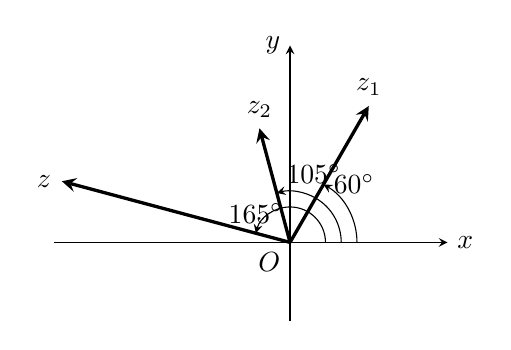
\begin{tikzpicture}[>=stealth]
 \draw[->](-3,0)--(2,0)node[right]{$x$};
    \draw[->](0,-1)--(0,2.5)node[left]{$y$};
    \node[below left]{$O$};
\draw[->,very thick](0,0)--(60:2)node[above]{$z_1$};
\draw[->,very thick](0,0)--(105:1.5)node[above]{$z_2$};
\draw[->,very thick](0,0)--(165:3)node[left]{$z$};    
\draw[->](.45,0)arc (0:165:.45)node[above=.15]{$165^{\circ}$};
\draw[->](.65,0)arc (0:105:.65)node[above right]{$105^{\circ}$};
\draw[->](.85,0)arc (0:60:.85)node[right=.2]{$60^{\circ}$};
\end{tikzpicture}
\captionof{figure}{}
\end{minipage}   


\begin{example}
    设$\vv{OZ}$表示$z=-1+i$。若$\vv{OZ}$逆时针旋转$120^{\circ}$,并伸长为原来的2倍得到$\vv{OZ_1}$,求$\vv{OZ_1}$表示的复数$z_1$.
\end{example}

\begin{solution}
    根据复数乘法的几何意义,设$z_1=z\cdot z_0$,其中
\[z_0=2(\pc{120^{\circ}})=2\left(-\frac{1}{2}+\frac{\sqrt{3}}{2}i\right)=-1+\sqrt{3}i\]
$\therefore\quad z_1=z\cdot z_0=(-1+i)\left(-1+\sqrt{3}i\right)=\left(1-\sqrt{3}\right)-\left(1+\sqrt{3}\right)i$
\end{solution}

\begin{rmk}
    从这个例子可以看出:欲求$z_1$,关键在于根据使$\vv{OZ}$旋转、拉长的条件正确地构造出“旋转伸缩因子”$z_0=r_0(\pc{\theta_0})$. 当旋转方向是逆时针时,$\theta_0>0$,当旋转方向是顺时针时,$\theta_0<0$,而$r_0$则是把$\vv{OZ}$拉长的倍数。特别地,
\begin{enumerate}[(1)]
\item 当$\vv{OZ}$长度不变,逆时针旋转$90^{\circ}$时,$z_0=\blank\blank$;
\item 当$\vv{OZ}$长度不变,顺时针旋转$90^{\circ}$时,$z_0=\blank\blank$.
\end{enumerate}
\end{rmk}

\begin{example}
如图6.23所示,$ABCD$是正方形,且已知$A$、$B$两点分别表示复数$2-i$和$3+3i$,求$C$、$D$两点表示的复数。
\end{example}

\begin{figure}[htp]
    \centering
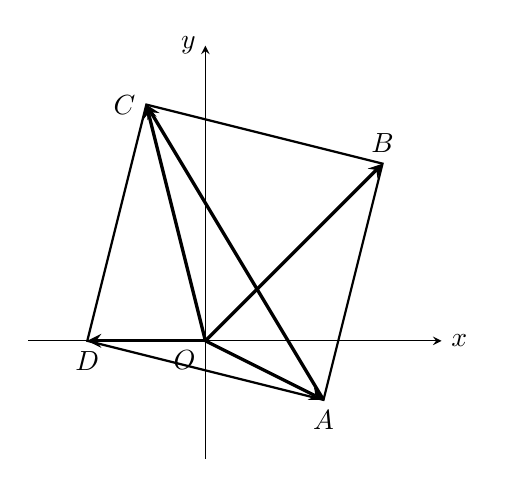
\begin{tikzpicture}[>=stealth, scale=.75]
    \draw[->](-3,0)--(4,0)node[right]{$x$};
    \draw[->](0,-2)--(0,5)node[left]{$y$};
    \node[below left]{$O$};
\draw[->,very thick](0,0)--(2,-1)node[below]{$A$};
\draw[->,very thick](0,0)--(3,3)node[above]{$B$};
\draw[->,very thick](0,0)--(-1,4)node[left]{$C$};    
\draw[->,very thick](0,0)--(-2,0)node[below]{$D$};    
\draw[thick](2,-1)--(3,3)--(-1,4)--(-2,0)--cycle;
\draw[->,very thick](2,-1)--(-1,4);

\end{tikzpicture}
    \caption{}
\end{figure}

\begin{solution}
$\because\quad z_{\vv{OA}}=2-i,\quad z_{\vv{OB}}=3+3i$

$\therefore\quad z_{\vv{AB}}=z_{\vv{OB}}-z_{\vv{OA}}=(3+3i)-(2-i)=1+4i$

由乘法的几何意义可知
\[\begin{split}
z_{\vv{AD}}&=z_{\vv{AB}}\cdot i=(1+4i)\cdot i =-4+i\\
z_{\vv{AC}}&=z_{\vv{AB}}\cdot \sqrt{2}\left(\pc{\frac{\pi}{4}}\right)=(1+4i)(1+i)=-3+5i
\end{split}\]

$\therefore\quad D$点表示的复数为
\[z_{\vv{OD}}=z_{\vv{OA}}+z_{\vv{AD}}=(2-i)+(-4+i)=-2\]
$C$点表示的复数为
\[z_{\vv{OC}}=z_{\vv{OA}}+z_{\vv{AC}}=(2-i)+(-3+5i)=-1+4i\]
\end{solution}

\begin{rmk}
\begin{enumerate}[(1)]
\item 本题在解决问题过程中,充分利用了复数加、减、乘法运算的几何意义,通过向量间的关系,找到了相关的复数间的关系,这是解决本问题的关键。
\item 复数乘法的几何意义,对于起点不在原点的向量也同样适用。
\item 判断向量的终点表示的复数是否是向量表示的复数时,应看向量的起点是否在原点,若向量的起点在原点,则向量终点表示的复数就是向量所表示的复数,否则就不是,这时只需再做一次加法运算就可以了,即加上向量的起点表示的复数。
\end{enumerate}
\end{rmk}

\begin{example}
如图6.24所示,平面上有三个并列而全等的正方形,利用复数证明$\angle 1+\angle 2+\angle 3=\frac{\pi}{2}$.
\end{example}

\begin{figure}[htp]
    \centering
\begin{tikzpicture}[>=stealth, scale=2]
    \draw[->](-.5,0)--(3.5,0)node[right]{$x$};
    \draw[->](0,-.5)--(0,1.5)node[left]{$y$};
    \node[below left]{$O$};
\draw(0,1)--(3,1);
\foreach \x in {1,2,3}
{
    \draw(\x,0)node[below]{\x}--(\x,1)node[above]{$Z_{\x}$};
}
\tkzDefPoints{0/0/O, 0/1/A, 1/1/B1, 2/1/B2, 3/1/B3}
\tkzDrawSegments(O,B1 O,B2 O,B3)
\tkzDrawPoints(B1,B2,B3)
\tkzMarkAngles[mark=none, size=.2cm](A,B1,O)
\tkzMarkAngles[mark=none, size=.3cm](A,B2,O)
\tkzMarkAngles[mark=none, size=.4cm](A,B3,O)
\tkzLabelAngle[pos=.3](A,B1,O){1}
\tkzLabelAngle[pos=.4](A,B2,O){2}
\tkzLabelAngle[pos=.5](A,B3,O){3}


\end{tikzpicture}
    \caption{}
\end{figure}

\begin{analyze}
    由复数乘法的几何意义可知,要想利用复数证明$\angle 1+\angle 2+\angle 3=\frac{\pi}{2}$,只需找出三个特定的复数$z_1,z_2,z_3$,使它们的辐角依次是$\angle 1, \angle 2, \angle 3$,那么乘积$z_1z_2z_3$的一个辐角就等于$\angle 1+\angle 2+\angle 3$,因此只需证明$z_1z_2z_3$所得复数的辐角只可能是$\frac{\pi}{2}$即可.
\end{analyze}

\begin{proof}
    如图6.24确定的复平面,利用两条直线平行内错角相等的定理,能使$\angle1,\angle2,\angle3$分别转化为复数$z_1=1+i$, $z_2=2+i$, $z_3=3+i$的辐角主值,于是
$$\angle1+\angle2+\angle3=\arg z_1+\arg z_2+\arg z_3$$

$\because\quad z_1\cdot z_2\cdot z_3=(1+i)(2+i)(3+i)=(1+3i)(3+i)=10i$

$\therefore\quad {\rm Arg\,}( z_1\cdot  z_2\cdot  z_3) = \frac \pi 2+ 2k\pi\quad ( k\in \Z)$\hfill (*) 

又$\because\quad 0<\arg z_{1}<\frac{\pi}{2},\quad 0<\arg z_{2}<\frac{\pi}{2},\quad 0<\arg z_{3}<\frac{\pi}{2}$

$\therefore\quad 0<\arg z_{1}+\arg z_{2}+\arg z_{3}<\frac{3\pi}{2}$,

$\therefore\quad \arg z_1+\arg z_2+\arg z_3=\frac\pi2$, [在(*)式中取$k=0$].

即$\angle 1+ \angle 2+ \angle 3= \frac \pi 2$ .
\end{proof}


\begin{example}
    利用复数计算
$\arcsin\frac{1}{\sqrt{10}}+\arccos\frac{5}{\sqrt{26}}+\arctan\frac{1}{7}+{\rm arccot\,}8$
\end{example}

\begin{solution}
我们分别以$\alpha,\beta,\gamma,\theta$标记上述四个角,不难看出
\[\alpha=\arg(3+i),\quad \beta=\arg(5+i),\quad \gamma=\arg(7+i),\quad \theta=\arg(8+i)\]
由于
$z=(3+i)(5+i)(7+i)(8+i)=650+650i$,
从而
\begin{equation}
    {\rm Arg\,}z=\pi+2k\pi,\; (k\in\Z)  \tag{*}
\end{equation}
但是,由于$\alpha,\beta,\gamma,\theta$都是锐角,

从而$0<\alpha+\beta+\gamma+\theta<2\pi$.

$\therefore\quad \alpha+\beta+\gamma+\theta=\frac{\pi}{4}$(在(*)式中,取$k=0$)
\end{solution}

\section*{习题七}
\begin{center}
    \bfseries A
\end{center}

\begin{enumerate}
    \item 把下列复数的三角形式写在横线上:
\begin{enumerate}[(1)]
    \item $\cos\theta-i\sin\theta = \blank\blank$
    \item $-(\pc{\theta}) = \blank\blank$
    \item $\sin\theta+i\cos\theta = \blank\blank$
    \item $\sin\theta-i\cos\theta = \blank\blank$
    \item $-\sin\theta-i\cos\theta = \blank\blank$
    \item $-\cos\theta+i\sin\theta = \blank\blank$
\end{enumerate}
    \item 计算:
\begin{enumerate}[(1)]
    \item $8\left(\pc{\frac{\pi}{6}}\right)\cdot 2\left(\pc{\frac{\pi}{4}}\right)$
    \item $2\left(\pc{\frac{4\pi}{3}}\right)\cdot 4\left(\pc{\frac{5\pi}{6}}\right)$
    \item $\sqrt{2}(\pc{240^{\circ}})\cdot \frac{\sqrt{3}}{2}(\pc{60^{\circ}})$
    \item $3\left(\pc{\frac{\pi}{3}}\right)\cdot 3\left(\pc{\frac{\pi}{6}}\right)$
    \item $\sqrt{10}\left(\pc{\frac{\pi}{2}}\right)\cdot \sqrt{2}\left(\pc{\frac{\pi}{4}}\right)$
    \item $3(\pc{18^{\circ}})\cdot 2(\pc{54^{\circ}})\cdot 5(\pc{108^{\circ}})$
    \item $\left[2(\pc{10^{\circ}})\right]^3$
    \item $5(\pc{30^{\circ}})\cdot 2\left[\pcx{-150^{\circ}}\right]$
    \item $(\cos\theta-i\sin\theta)\cdot (\cos2\theta-i\sin2\theta)$
    \item $(-\cos\theta-i\sin\theta)\cdot (\sin\theta-i\cos\theta)$
\end{enumerate}
    \item 在直角坐标系中,已知$A(1,1)$, $B(2,2)$,求:
\begin{enumerate}[(1)]
\item 以$AB$为边的正方形的其余两顶点坐标;
\item 以$AB$为斜边的等腰直角三角形$ABM$的顶点$M$的坐标。 
\end{enumerate}
\item 
把与复数$3-\sqrt{3}i$对应的向量按顺时针方向旋转$60^{\circ}$,求与所得的向量对应的复数。
\item 直角三角形$ABC$中,$\angle C=\frac{\pi}{2}$,$BC=\frac{1}{3}AC$,点$E$在$AC$
上,且$EC=2AE$,利用复数证明$\angle CBE+\angle CBA=\frac{3\pi}{4}$.

\item 如图$ABCD$是边长为$a$的正方形,$OB=2a$,用复数证明$\angle AOB+\angle DOC=\frac{\pi}{4}$。
\begin{figure}[htp]
    \centering
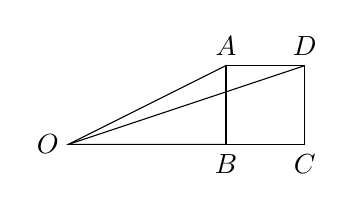
\begin{tikzpicture}
\draw(-2,0)node[left]{$O$}--(0,1)node[above]{$A$}--(0,0)node[below]{$B$}--cycle;
\draw(0,0)rectangle (1,1)node[above]{$D$};
\draw(-2,0)--(1,1);
\node at (1,0)[below]{$C$};
\end{tikzpicture}
    \caption*{第6题}
\end{figure}
\end{enumerate}


\begin{center}
    \bfseries B
\end{center}

\begin{enumerate}\setcounter{enumi}{6}
\item 把模相等的两个复数$z_1$,$z_2$对应的向量$\vv{OA}$, $\vv{OB}$分别逆时针旋转$\frac{\pi}{4}$和$\frac{5\pi}{3}$后,与向量$\vv{OM}$重合。已知$z_2=-1-\sqrt{3}i$, 求$z_1$的代数形式和$\arg z_1$。
\item 用两种方法证明(或求值):
\begin{enumerate}[(1)]
    \item $\arcsin\frac{4}{5}+2\arctan\frac{1}{3}=\frac{\pi}{2}$
    \item $\arctan(-2)+\arctan(-3)=?$
\end{enumerate}

\item 计算
$\arcsin\frac{1}{\sqrt{10}}+\arcsin\frac{1}{\sqrt{50}}+\arctan\frac{7}{31}+{\rm arccot\,}10$

\item $\alpha,\beta$均为锐角,且$\tan\alpha=\frac{1}{7}$,$\sin\beta=\frac{1}{\sqrt{10}}$,求证$\alpha+2\beta=\frac{\pi}{4}$.
\item 设$\arg(1-3i)=\alpha$, $\arg(3-i)=\beta$,求$\alpha+\beta$.
\end{enumerate}